\documentclass[10pt,a4paper]{article}
\usepackage{iftex}
\ifPDFTeX
  \usepackage[T1]{fontenc}
  \usepackage[utf8]{inputenc}
\fi
\usepackage{lmodern}
\usepackage[a4paper,left=23mm,right=23mm,top=24mm,bottom=24mm]{geometry}
\usepackage{amsmath,amssymb,amsthm,mathtools}
\usepackage{booktabs,array,enumitem,microtype,fancyhdr,float,graphicx,xcolor,placeins}
\usepackage[font=small,labelfont=bf]{caption}
\usepackage{tikz}
\usetikzlibrary{calc,arrows.meta,positioning,fit,backgrounds,shapes.geometric}
\usepackage[colorlinks=true,linkcolor=blue!45!black,citecolor=blue!45!black,urlcolor=blue!45!black]{hyperref}
\hypersetup{pdfauthor={Ivan Besevic},pdftitle={The Simultaneous Rectangle (G8, revision 10)}}

% ---- Unified V31 / C5 / G8 editorial palette ----
\definecolor{ink}{RGB}{28,36,48}
\definecolor{supp}{RGB}{22,82,158}
\definecolor{trans}{RGB}{21,128,82}
\definecolor{acc}{RGB}{210,88,18}
\definecolor{tealc}{RGB}{13,132,148}
\definecolor{plum}{RGB}{128,42,138}
\definecolor{slatec}{RGB}{110,124,142}
\definecolor{rectfill}{RGB}{246,249,253}
\definecolor{bluefill}{RGB}{236,244,252}
\definecolor{greenfill}{RGB}{236,249,242}
\definecolor{trifill}{RGB}{254,242,230}

\pagestyle{fancy}\fancyhf{}
\fancyhead[L]{\small\textcolor{slatec}{Geometric root calculators: the simultaneous rectangle}}
\fancyhead[R]{\small\textcolor{slatec}{G8 rev.\ 10 / Research preprint}}
\fancyfoot[C]{\small\thepage}
\renewcommand{\headrulewidth}{0.3pt}
\setlength{\parindent}{0pt}\setlength{\parskip}{5pt plus 1pt}
\setlist{itemsep=1.5pt,topsep=2.5pt}
\setlength{\emergencystretch}{2em}

\newtheorem{theorem}{Theorem}[section]
\newtheorem{lemma}[theorem]{Lemma}
\newtheorem{proposition}[theorem]{Proposition}
\newtheorem{corollary}[theorem]{Corollary}
\theoremstyle{definition}
\newtheorem{definition}[theorem]{Definition}
\newtheorem{remark}[theorem]{Remark}
\numberwithin{equation}{section}

\newcommand{\R}{\mathbb{R}}
\newcommand{\C}{\mathbb{C}}

% Clean V31-style callout box for key ideas
\newcommand{\keyidea}[2]{%
  \par\vspace{3pt}\noindent
  \begin{tikzpicture}
    \node[anchor=north west,inner xsep=10pt,inner ysep=7pt,text width=\dimexpr\linewidth-24pt\relax,
          fill=rectfill,rounded corners=2pt,draw=slatec!28,line width=0.45pt] (box)
          {\small\textcolor{supp}{\textbf{#1.}}\enspace #2};
    \fill[supp] (box.north west) rectangle ([xshift=2.6pt]box.south west);
  \end{tikzpicture}\par\vspace{3pt}%
}

\begin{document}

\noindent\textcolor{supp}{\rule{\linewidth}{1.6pt}}
\vspace{4pt}

{\small\scshape\textcolor{slatec}{Constructive geometry \,/\, root iterations \,/\, all roots, one method}}

\vspace{5pt}
{\LARGE\bfseries\textcolor{ink}{The simultaneous rectangle}\par}
\vspace{3pt}
{\large\raggedright\textcolor{ink!85}{All the roots by the rectangle alone: the three means used twice per sweep, one certificate, no rescue path}\par}
\vspace{8pt}
Ivan Besevic\footnote{Computational assistance: AI was used for derivations, proofs, numerical experiments, figures and manuscript preparation. The author is responsible for the claims and their attribution. Section~\ref{sec:evidence} states which results are formal proofs, written proofs, and numerical observations.}
\quad$\cdot$\quad Independent research\\
Version G8, revision 10 (crate \texttt{pandroots} 0.30.0: C5 slit-plane branch, $O(m)$ disjoint-disc three-mean pre-polish, multi-pass exact sweeps, local zoom beyond $2^{-500}$, 100\,000-polynomial benchmark) \quad$\cdot$\quad \mbox{23 November 2026}\\
\url{https://crates.io/crates/pandroots} \quad$\cdot$\quad \url{https://github.com/ivan-fr/pandrosion}

\vspace{6pt}
\begin{quote}\small
\textbf{Abstract.}
The fast path of~\cite{g7} finds the roots of a polynomial by the Ehrlich--Aberth iteration and keeps the Pandrosion rectangle of~\cite{v31} only in two rescue methods. This note puts the rectangle back at the centre and removes all rescue paths. The Ehrlich--Aberth step is Newton's step on the polynomial deflated of the other approximations, that is, the line $AK$ of the rectangle on that deflated function. Replacing $AK$ by the three-mean support $q_M(t)$ gives a simultaneous iteration of order~4; if, in addition, every neighbour is seen where the three-mean step of~\cite{g2} announces it, the order is~6 (Theorem~\ref{thm:order}). The same theorem shows that the leading error term does not depend on the support: the order~9 of~\cite{v31} does not transfer, and the three means do no better locally than the conic support. Evaluated on its natural slit-plane branch holomorphic on $\C\setminus(-\infty,0]$ (\cite{c5}, Theorem~3.8), $q_M(t)$ avoids the spurious vertical branch cut of the naive principal-root formula in both double precision and multiprecision.

The points start from the dominant binomials of the Newton polygon at every scale (Section~\ref{sec:start}), saving 9 to 33\,\% of sweeps on random polynomials and most sweeps on multi-scale polynomials; pairwise-disjoint safety discs read in $O(m)$ from the start further enable an $O(m)$ three-mean pre-polish before any $O(m^2)$ reciprocal sums are formed. The certificate is read on the same deflated values: Smith's discs~\cite{smith} enclose all roots, and a contraction argument proves that $D(z_k,2|W_k|)$ contains exactly one of them (Theorem~\ref{thm:fp}). Whenever a disc does not yet satisfy the tolerance or real-root criterion, the same sweep continues with exact fixed-point ball evaluations, multi-pass Gauss--Seidel updates, arbitrary-precision dyadic points, a shifted-power cluster step (Section~\ref{sec:cluster}), and a local change of variable (\texttt{zoom}) isolating roots down to $2^{-8000}$ apart.

The zero-\texttt{unsafe} Rust crate \texttt{pandroots} (version 0.30.0, 80 tests) certifies all roots up to 203 times faster than \texttt{numpy.roots}/LAPACK computes uncertified eigenvalues at degree~320 (553\,$\mu$s against 112\,ms, complex coefficients; 48 times faster for real coefficients), and at degree~320 the three-mean rectangle now outperforms Ehrlich--Aberth in wall-clock time as well as sweeps (554\,$\mu$s against 743\,$\mu$s). On a 100\,000-polynomial corpus spanning sixteen families (5\,060\,069 roots, degrees up to 2000), version 0.30.0 completes in 16.50\,s on one Apple~M5 thread (1.83$\times$ faster than 0.28.0 and 1.18$\times$ faster than 0.29.0), certifying 100\,000/100\,000 polynomials completely and passing all 36\,000/36\,000 exact rational oracles with zero failures.
\emph{Limits:} no proof of global convergence; a symmetric trap for real polynomials left by rounding only (Section~\ref{sec:trap}); iterations of this structure and Newton-polygon starts exist in the literature~\cite{hpr,ppz,prp,bini}; non-dyadic clusters closer than $\sim 2^{-16000}$ remain grouped. The core mathematics is formalised in Lean~4 across ten modules (84 theorems, no \texttt{sorry}, standard axioms only, Section~\ref{sec:evidence}), complemented by an Aeneas-extracted dyadic verifier; the Rust floating-point rounding bounds, ball evaluation, and full executable remain outside the formal proof.
\end{quote}

\vspace{2pt}\noindent\textcolor{slatec!40}{\rule{\linewidth}{0.5pt}}

% =========================================================================
\section{Purpose}\label{sec:purpose}
The note~\cite{g7} separated the search from the proof: any method may propose candidates, a certificate decides. Its search was the Ehrlich--Aberth iteration~\cite{ehrlich,aberth}, its certificate had two layers, and two other methods (the descent of~\cite{g3}, the subdivision of~\cite{g6}) took over when a certificate failed. The step of~\cite{v31,g2} was no longer on the main path. Two requirements are set here: the search must be a rectangle iteration driven by the three-mean support $q_M(t)$, and the code must follow one unified path without rescue methods.

The starting point is an identity. For approximations $z_1,\dots,z_m$ of the roots of $S$, the Ehrlich--Aberth step is Newton's step for $F_k(w)=S(w)/\prod_{l\ne k}(w-z_l)$ at $z_k$; and Newton's step is the rectangle step with the line $AK$ as support~\cite{v31,g2}. So the other supports of the rectangle---in particular the three-mean support $q_M(t)$---can be applied to $F_k$ as well.

\begin{figure}[!htbp]\centering
\resizebox{\textwidth}{!}{%
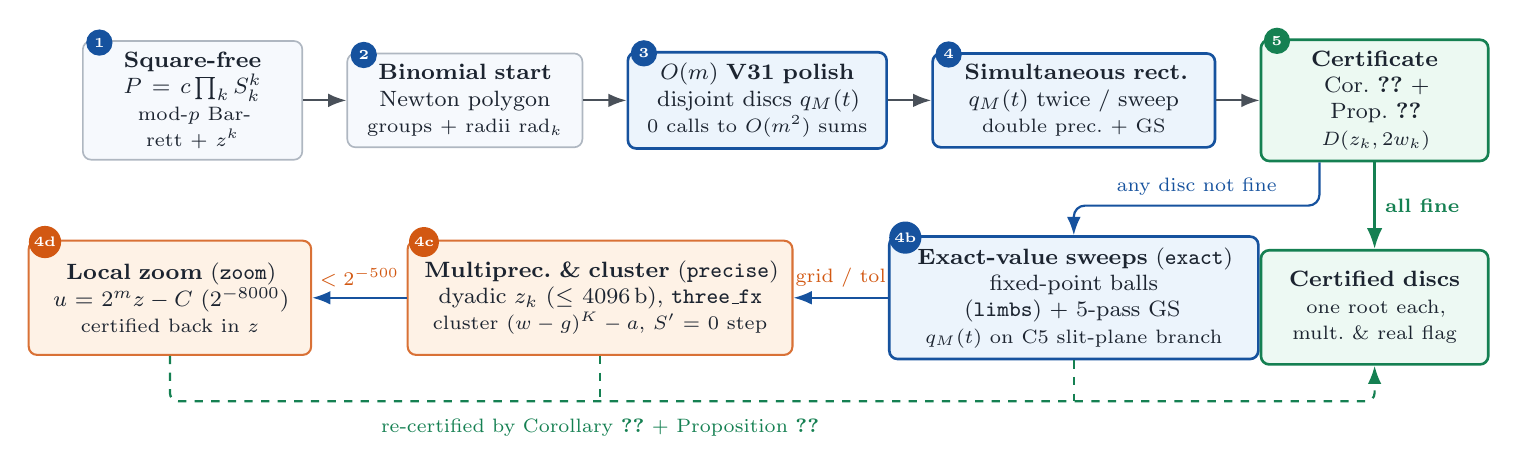
\begin{tikzpicture}[
  >=Latex,
  node distance=5mm and 5.5mm,
  stage/.style={rectangle,rounded corners=3pt,draw=slatec!55,fill=rectfill,line width=0.6pt,
                minimum height=11.5mm,inner xsep=5.5pt,inner ysep=4pt,align=center,font=\footnotesize,text=ink},
  core/.style={stage,draw=supp,fill=bluefill,line width=0.95pt},
  cert/.style={stage,draw=trans,fill=greenfill,line width=0.95pt},
  esc/.style={stage,draw=acc!85,fill=trifill,line width=0.75pt},
  badge/.style={circle,fill=supp,text=white,font=\tiny\bfseries,inner sep=1.1pt,minimum size=9.5pt},
  badgeg/.style={badge,fill=trans},
  badgea/.style={badge,fill=acc},
  arr/.style={->,line width=0.8pt,ink!80},
  looparr/.style={->,line width=0.8pt,supp,rounded corners=4pt}
]
% Top row: main pipeline
\node[stage,text width=24mm] (sqf) {\textbf{Square-free}\\$P = c\prod_k S_k^k$\\{\scriptsize mod-$p$ Barrett + $z^k$}};
\node[stage,right=of sqf,text width=26mm] (start) {\textbf{Binomial start}\\Newton polygon\\{\scriptsize groups + radii $\mathrm{rad}_k$}};
\node[core,right=of start,text width=29mm] (v31) {\textbf{$O(m)$ V31 polish}\\disjoint discs $q_M(t)$\\{\scriptsize 0 calls to $O(m^2)$ sums}};
\node[core,right=of v31,text width=32mm] (rect) {\textbf{Simultaneous rect.}\\$q_M(t)$ twice / sweep\\{\scriptsize double prec.\ + GS}};
\node[cert,right=of rect,text width=25mm] (cert) {\textbf{Certificate}\\Cor.~\ref{cor:fp} + Prop.~\ref{prop:real}\\{\scriptsize $D(z_k,2w_k)$}};

% Badges
\node[badge] at ($(sqf.north west)+(2.2mm,-0.3mm)$) {1};
\node[badge] at ($(start.north west)+(2.2mm,-0.3mm)$) {2};
\node[badge] at ($(v31.north west)+(2.2mm,-0.3mm)$) {3};
\node[badge] at ($(rect.north west)+(2.2mm,-0.3mm)$) {4};
\node[badgeg] at ($(cert.north west)+(2.2mm,-0.3mm)$) {5};

% Bottom row: precision escalation (uniform 3-line height, generous arrow gaps, zero crossing arrows)
\node[core,below=11mm of rect,text width=43mm,minimum height=14.5mm] (exact) {\textbf{Exact-value sweeps} (\texttt{exact})\\fixed-point balls (\texttt{limbs}) + 5-pass GS\\{\scriptsize $q_M(t)$ on C5 slit-plane branch}};
\node[esc,left=12mm of exact,text width=45mm,minimum height=14.5mm] (prec) {\textbf{Multiprec.\ \& cluster} (\texttt{precise})\\dyadic $z_k$ ($\le 4096$\,b), \texttt{three\_fx}\\{\scriptsize cluster $(w-g)^K-a$, $S'=0$ step}};
\node[esc,left=12mm of prec,text width=32mm,minimum height=14.5mm] (zoom) {\textbf{Local zoom} (\texttt{zoom})\\$u = 2^m z - C$ ($2^{-8000}$)\\{\scriptsize certified back in $z$}};

\node[badge] at ($(exact.north west)+(2.2mm,-0.3mm)$) {4b};
\node[badgea] at ($(prec.north west)+(2.2mm,-0.3mm)$) {4c};
\node[badgea] at ($(zoom.north west)+(2.2mm,-0.3mm)$) {4d};

% Certified output box directly below Certificate (same row as bottom escalation stages!)
\node[cert,below=11mm of cert,text width=25mm,minimum height=14.5mm,fill=greenfill!95] (done) {\textbf{Certified discs}\\{\scriptsize one root each,}\\{\scriptsize mult.\ \& real flag}};

% Arrows top row
\draw[arr] (sqf) -- (start);
\draw[arr] (start) -- (v31);
\draw[arr] (v31) -- (rect);
\draw[arr] (rect) -- (cert);

% Fast exit arrow: straight down from Certificate right side into Certified discs
\draw[->,line width=1.0pt,trans] (cert.south) -- node[right,font=\scriptsize\bfseries,text=trans]{all fine} (done.north);

% Escalation feedback loop: drops from Certificate left-of-centre into the corridor, then down into Exact-value sweeps
\coordinate (esc_turn) at ([xshift=-7mm,yshift=-5.5mm]cert.south);
\draw[looparr] ([xshift=-7mm]cert.south) -- (esc_turn) -| node[pos=0.25,above,font=\scriptsize,text=supp]{any disc not fine} (exact.north);
\draw[looparr] (exact.west) -- node[above,font=\scriptsize,text=acc]{grid / tol} (prec.east);
\draw[looparr] (prec.west) -- node[above,font=\scriptsize,text=acc]{$<2^{-500}$} (zoom.east);

% Clean shared return bus underneath all three escalation boxes into Certified discs
\coordinate (bus_y) at ([yshift=-5.2mm]exact.south);
\draw[->,line width=0.8pt,trans,dashed,rounded corners=3pt] (zoom.south) -- (zoom.south |- bus_y) -| (done.south);
\draw[line width=0.8pt,trans,dashed] (prec.south) -- (prec.south |- bus_y);
\draw[line width=0.8pt,trans,dashed] (exact.south) -- (exact.south |- bus_y);
\node[below=1.0mm of $(prec.south |- bus_y)$,font=\scriptsize,text=trans] {re-certified by Corollary~\ref{cor:fp} + Proposition~\ref{prop:real}};

\end{tikzpicture}%
}
\caption{Single-path architecture of \texttt{pandroots 0.30.0}. Every search stage (shaded cobalt) runs the same three-mean support $q_M(t)$ of~\cite{v31,c5}, escalating only the arithmetic precision and local coordinates when the a posteriori fixed-point certificate (emerald) asks for sharper bounds. There is no rescue solver.}\label{fig:arch}
\end{figure}

Contents of the paper:
\begin{itemize}
\item Section~\ref{sec:step}: the deflated rectangle step, its C5 slit-plane branch, and its double use per sweep.
\item Section~\ref{sec:order}: local orders 3, 4, 5, 6, and why the order~9 of~\cite{v31} collapses at $t=1$.
\item Section~\ref{sec:cert}: the unified fixed-point certificate and precision continuation.
\item Section~\ref{sec:start}: the dominant-binomial start and the $O(m)$ disjoint-disc V31 pre-polish (0.30.0).
\item Sections~\ref{sec:algo} to~\ref{sec:meas}: the algorithm, the symmetric trap for real polynomials, and prototype measurements.
\item Section~\ref{sec:rust}: the Rust crate \texttt{pandroots} from 0.1.0 to 0.30.0, including the 100\,000-polynomial benchmark.
\item Section~\ref{sec:cluster}: clusters, zeros of $S'$, and local variable zoom beyond $2^{-500}$.
\item Section~\ref{sec:evidence}: Lean~4 formalisation (84 theorems across ten modules), independent checks, and limits.
\end{itemize}
Throughout, $S$ is a square-free polynomial of degree $m\ge2$ with leading coefficient $c$ and roots $\zeta_1,\dots,\zeta_m$; multiplicities are removed beforehand by the exact square-free decomposition~\cite{g5,g6}.

% =========================================================================
\section{The rectangle on the deflated function}\label{sec:step}
\textbf{Supports and the C5 slit-plane branch.}
A \emph{support} is a function $q$ of the cursor $t$ with $q(1)=1$. Those of~\cite{v31} used here are the line $AK$, $q=1$; the line $AD$, $q=(1+t)/2$; the conic $q=\sqrt t$; and the \emph{three means of degree $p$},
\begin{equation}\label{eq:qm_direct}
 q_M(t)=\mu(1+t)+\gamma\sqrt t-\nu\sqrt{t+\delta(t-1)^2},\qquad
 \begin{aligned}
 \mu&=\tfrac{(p-2)(47p^2+21p+4)}{60p(4p^2-1)}, & \gamma&=\tfrac{16(p+1)(4p^2-1)}{15p(5p^2+4)},\\
 \nu&=\tfrac{49p(p+1)(p^2-4)}{10(4p^2-1)(5p^2+4)}, & \delta&=\tfrac{5p^2+4}{84p^2}.
 \end{aligned}
\end{equation}
On the right half-plane $\operatorname{Re} t\ge 0$, taking principal square roots in~\eqref{eq:qm_direct} is holomorphic; however, because $t+\delta(t-1)^2$ crosses $(-\infty,0]$ whenever $\operatorname{Re} t = 1 - \frac{1}{2\delta}$ (for instance $\operatorname{Re} t \approx -7.33$ at $p=10$), the naive form~\eqref{eq:qm_direct} exhibits a spurious vertical branch cut in the left half-plane. By Theorem~3.8 of~\cite{c5}, factoring $z=\sqrt{t}$ (principal square root, $\operatorname{Re} z>0$ on $\C\setminus(-\infty,0]$) yields the \emph{natural slit-plane branch}
\begin{equation}\label{eq:qm_slit}
 q_M(t)=z\Bigl(\mu\bigl(z+z^{-1}\bigr)+\gamma-\nu\sqrt{1+\delta\bigl(z-z^{-1}\bigr)^2}\Bigr),
\end{equation}
which agrees with~\eqref{eq:qm_direct} on $\operatorname{Re} t\ge 0$ and extends holomorphically to the entire slit plane $\C\setminus(-\infty,0]$ (Figure~\ref{fig:basins}, bottom row). For $|t|\ge 10^{140}$ the asymptotic expansion $q_M(t)=(\mu-\nu\sqrt{\delta})\,t+\gamma\sqrt{t}+O(1)$ avoids squaring overflow. Since \texttt{pandroots} 0.29.0 (double precision) and 0.30.0 (multiprecision \texttt{three\_fx}), both paths evaluate~\eqref{eq:qm_slit} whenever $\operatorname{Re} t<0$.

For a function $f$ at a point $z$, with $N=f/f'$ and $L=ff''/f'^2$, the virtual-anchor step of degree $p$ of~\cite{g2} is
\begin{equation}\label{eq:g2}
 t=1-\frac{p}{p-1}\,L,\qquad z^+=z-\frac{p\,N}{1+(p-1)\,q(t)} .
\end{equation}
With $q=1$ it is Newton's step, with the line $AD$ Halley's, with the conic and $p=\deg f$ Laguerre's, and with $q=q_M$ the three-mean step.

\begin{definition}\label{def:defl}
Let $z_1,\dots,z_m$ be distinct and let $y_1,\dots,y_m$ be \emph{announced positions} ($y_l=z_l$ if nothing is announced). The function deflated for the index $k$ is $F_k(w)=S(w)\big/\prod_{l\ne k}(w-y_l)$, and
\begin{equation}\label{eq:AB}
 A_k=\frac{S'(z_k)}{S(z_k)}-\sum_{l\ne k}\frac1{z_k-y_l},\qquad
 B_k=\frac{S'(z_k)^2-S(z_k)S''(z_k)}{S(z_k)^2}-\sum_{l\ne k}\frac1{(z_k-y_l)^2}.
\end{equation}
\end{definition}

\begin{proposition}\label{prop:step}
$A_k=F_k'/F_k$ and $B_k=-(F_k'/F_k)'$ at $z_k$. The step~\eqref{eq:g2} applied to $F_k$ at $z_k$ is
\begin{equation}\label{eq:step}
 t_k=\frac{pB_k-A_k^2}{(p-1)A_k^2},\qquad z_k^+=z_k-\frac{p}{A_k\,\bigl(1+(p-1)\,q(t_k)\bigr)} .
\end{equation}
With $q=1$ and $y=z$ it is the Ehrlich--Aberth step $z_k-1/A_k$.
\end{proposition}
\begin{proof}
The logarithmic derivative of $F_k$ is $S'/S-\sum_{l\ne k}1/(w-y_l)$; differentiating once more gives $B_k$. Then $N=1/A_k$ and $F_k''/F_k=A_k^2-B_k$, so $L=1-B_k/A_k^2$ and $t=1-\frac{p}{p-1}(1-B_k/A_k^2)$, which is~\eqref{eq:step}. For $q=1$ the denominator is $pA_k$.
\end{proof}

\begin{definition}[Simultaneous rectangle]\label{def:sweep}
One sweep, from distinct points $z_1,\dots,z_m$:
\begin{enumerate}
\item \emph{announce:} $y_l=z_l-h_l$, where $h_l$ is the step~\eqref{eq:g2} for $f=S$ at $z_l$ with $p=m$ and the three means~\eqref{eq:qm_slit};
\item \emph{move:} $z_k^+$ by~\eqref{eq:step} with $p=m$ and the three means, for every $k$ (in Gauss--Seidel order in the Rust crate, updating $y_k\leftarrow z_k^+$ immediately).
\end{enumerate}
\end{definition}
The same support, of the same degree, is used twice: once on $S$, once on $S$ deflated. A sweep needs $S,S',S''$ at the $m$ points, $m^2$ complex divisions for the two sums of~\eqref{eq:AB}, and $4m$ square roots.

\begin{figure}[!htbp]\centering
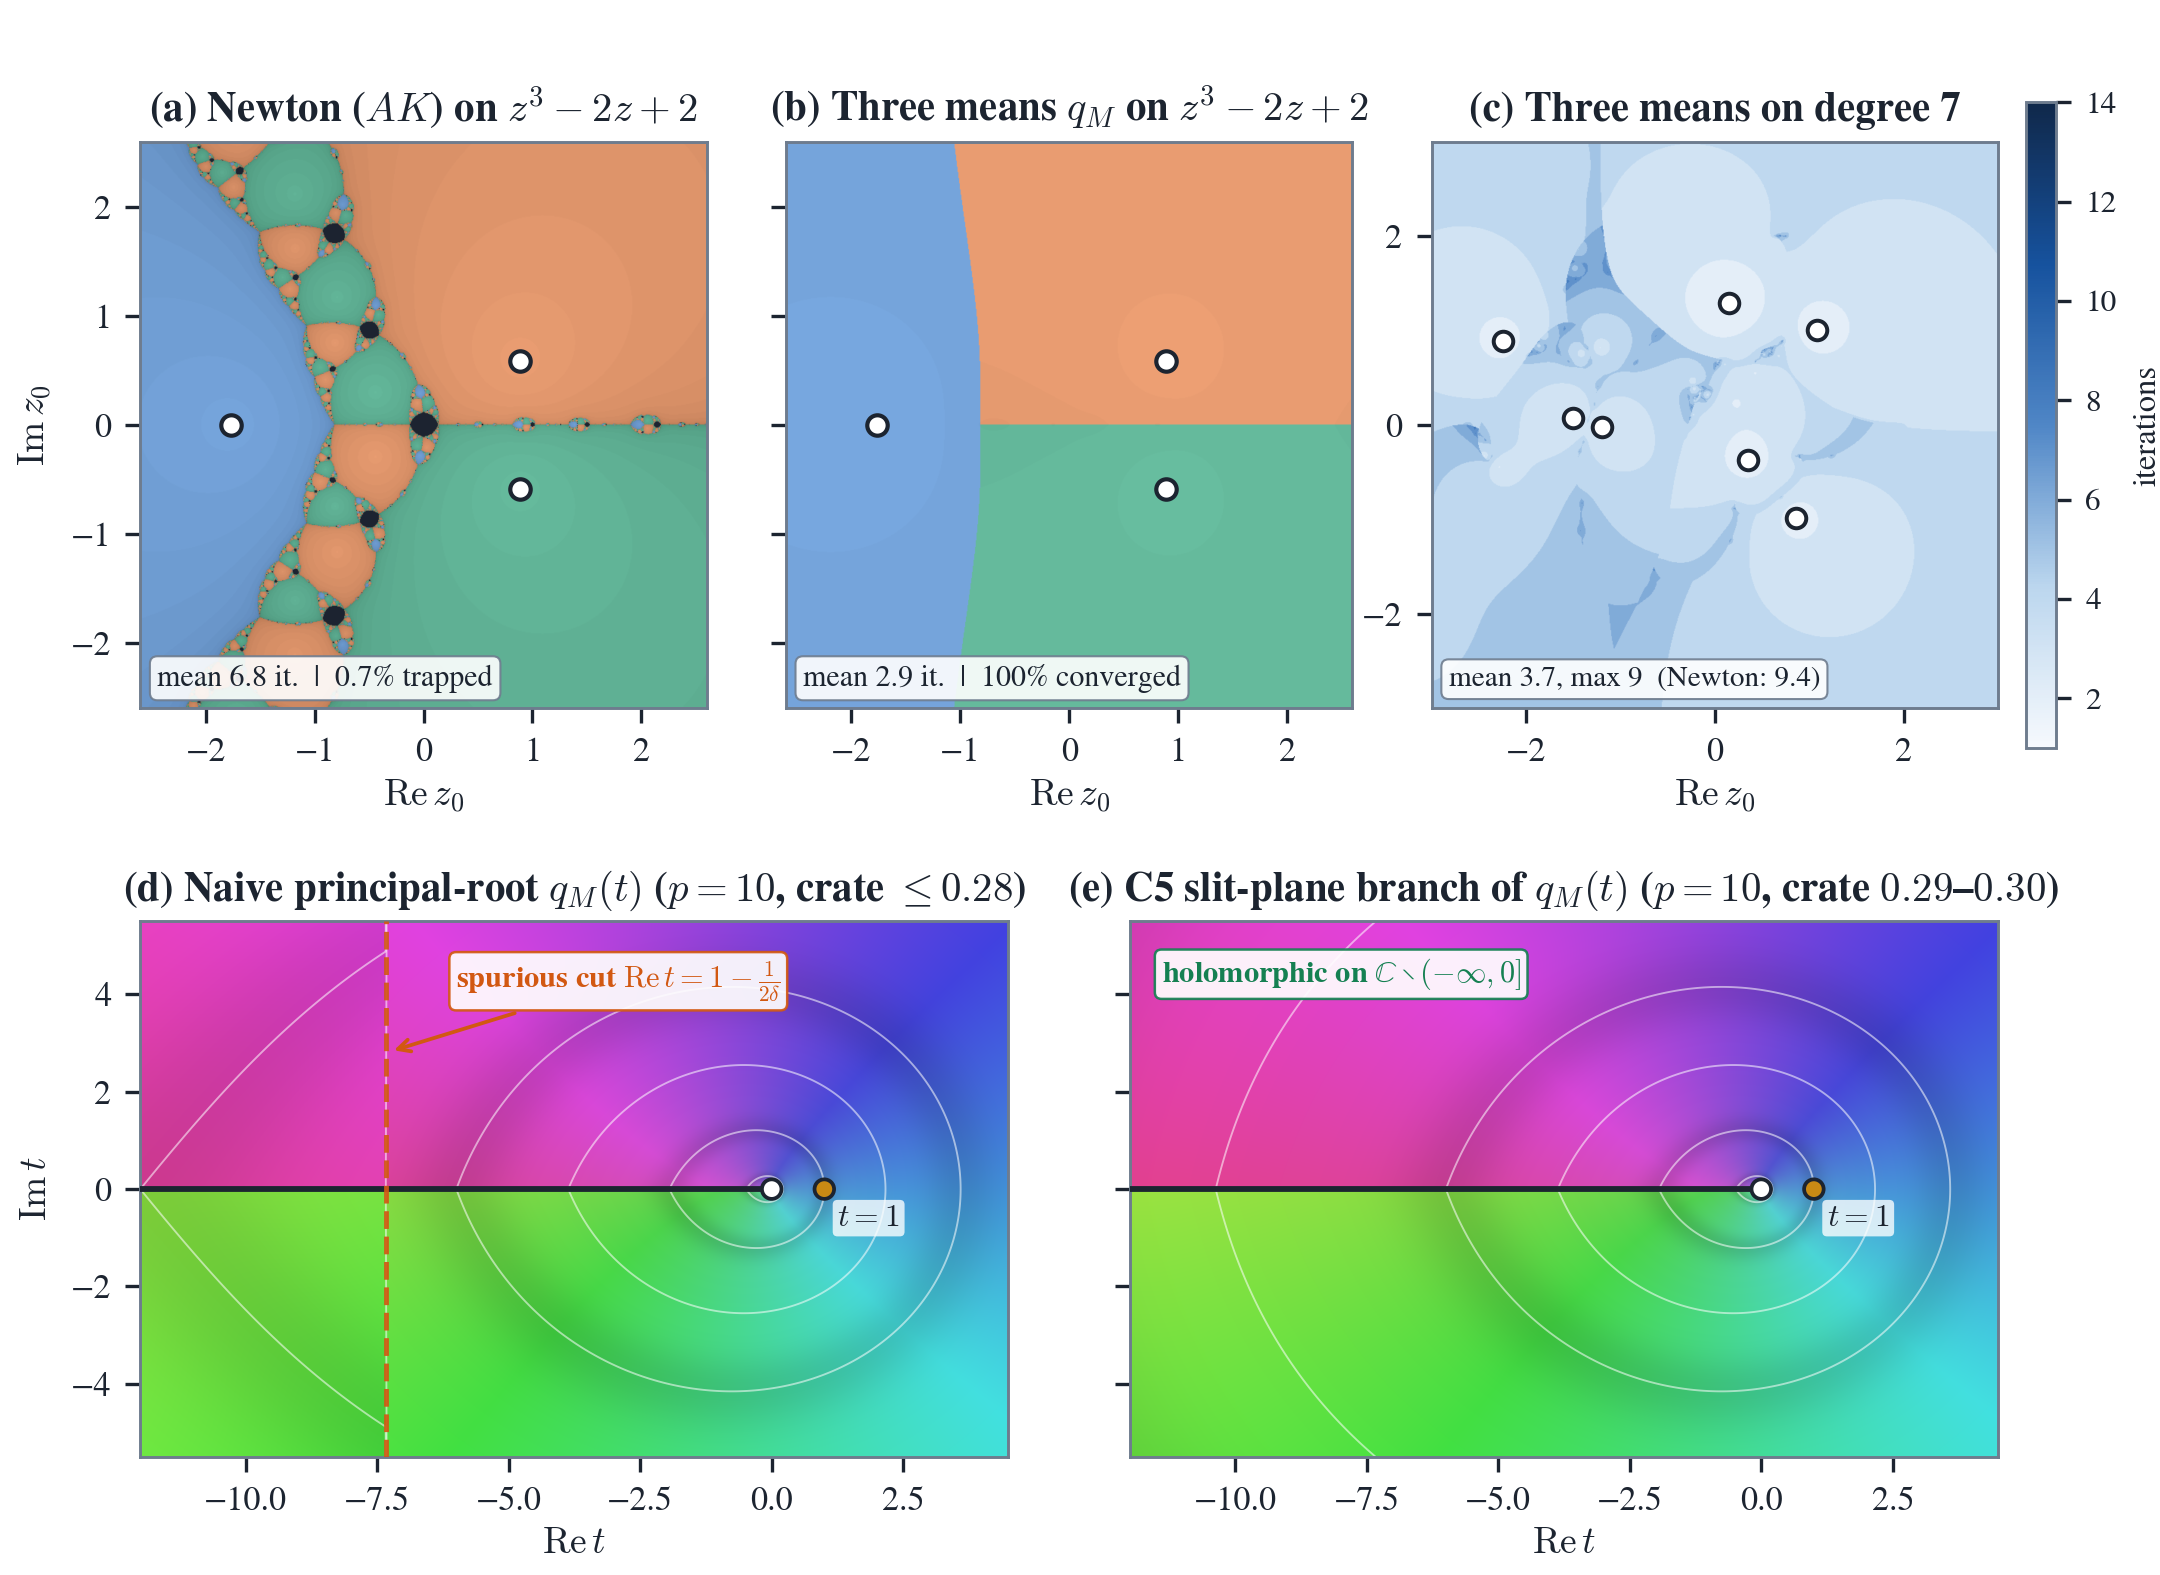
\includegraphics[width=\textwidth]{fig_basins_slit.png}
\caption{The three-mean support in action and its C5 slit-plane branch. \textbf{Top:} single-root iteration~\eqref{eq:g2} from every starting point $z_0$ ($750\times 750$ grid; white dots: roots). (a)~Newton's step ($AK$) on $z^3-2z+2$: fractal basin boundaries and the attracting 2-cycle $0\leftrightarrow 1$ (black, 0.7\,\% of the window). (b)~Three-mean step $q_M$ on $z^3-2z+2$: clean basins, 100\,\% convergence, mean 2.9 iterations (Newton: 6.8). (c)~Iteration count of $q_M$ on a degree-7 complex polynomial (mean 3.7, max 9; Newton: 9.4). \textbf{Bottom:} complex domain colouring (hue = $\arg q_M(t)$, white contours = $|q_M(t)|$) for $p=10$. (d)~The naive principal-root formula~\eqref{eq:qm_direct} introduces a spurious vertical branch cut along $\operatorname{Re} t = 1-1/(2\delta)\approx -7.33$. (e)~The C5 Theorem~3.8 slit-plane branch~\eqref{eq:qm_slit} removes the spurious cut completely, leaving $q_M$ holomorphic on $\C\setminus(-\infty,0]$.}\label{fig:basins}
\end{figure}

% =========================================================================
\section{Local order}\label{sec:order}
Let $e_k=z_k-\zeta_k$, $\eta_l=y_l-\zeta_l$, $\varepsilon=\max|e_k|$, $\eta=\max|\eta_l|$, and
\[
 \delta_1=\sum_{l\ne k}\Bigl(\frac1{z_k-\zeta_l}-\frac1{z_k-y_l}\Bigr),\qquad
 \delta_2=\sum_{l\ne k}\Bigl(\frac1{(z_k-\zeta_l)^2}-\frac1{(z_k-y_l)^2}\Bigr),
\]
both $O(\eta)$ when the roots are simple and the points close to them.

\begin{theorem}\label{thm:order}
Let $q$ be analytic near $1$ with $q(1)=1$, $q'(1)=\frac12$, $q''(1)=2q_2$, and let $p>1$. With $x=\delta_1e_k$ and $v=\delta_2e_k^2$, the step~\eqref{eq:step} satisfies
\begin{equation}\label{eq:err}
 \frac{e_k^+}{e_k}=\frac{v}{2}+\Bigl(\frac12+\frac{4p\,q_2}{p-1}\Bigr)x^2+O\bigl(|x|^3+|xv|+|v|^2\bigr),
 \qquad\text{while for }q=1:\quad\frac{e_k^+}{e_k}=\frac{x}{1+x}.
\end{equation}
\end{theorem}
\begin{proof}
Since $S'/S=\sum_l 1/(w-\zeta_l)$ and $(S'^2-SS'')/S^2=\sum_l 1/(w-\zeta_l)^2$,~\eqref{eq:AB} gives $A_k=(1+x)/e_k$ and $B_k=(1+v)/e_k^2$. Hence $t_k-1=\dfrac{p\,(v-2x-x^2)}{(p-1)(1+x)^2}$ and $\dfrac{e_k^+}{e_k}=1-\dfrac{p}{(1+x)\bigl(1+(p-1)q(t_k)\bigr)}$. For $q=1$ this is $x/(1+x)$. Otherwise $(p-1)q(t_k)=p-1+\frac{p(v-2x-x^2)}{2(1+x)^2}+\frac{p^2q_2}{p-1}\frac{(v-2x-x^2)^2}{(1+x)^4}+\dots$, so that
\[
 (1+x)\bigl(1+(p-1)q(t_k)\bigr)=p\Bigl[1+\frac{x^2+v}{2(1+x)}+\frac{4p\,q_2}{p-1}x^2+\dots\Bigr],
\]
and~\eqref{eq:err} follows; the term in $x$ alone cancels.
\end{proof}

\begin{corollary}\label{cor:order}
Near simple roots, with all errors of the same size:
\begin{center}\small
\begin{tabular}{llll}
\toprule
support on $F_k$ & announced positions & leading error & order\\
\midrule
$AK$ & none ($y=z$) & $\delta_1 e_k^2$ & 3 (Ehrlich--Aberth)\\
$AK$ & step of order 3 on $S$ & $\delta_1 e_k^2$, $\delta_1=O(\varepsilon^3)$ & 5\\
any $q$ with $q'(1)=\frac12$ & none & $\frac12\delta_2 e_k^3$ & 4\\
any $q$ with $q'(1)=\frac12$ & step of order 3 on $S$ & $\frac12\delta_2 e_k^3$, $\delta_2=O(\varepsilon^3)$ & 6\\
\bottomrule
\end{tabular}
\end{center}
The sweep of Definition~\ref{def:sweep} has order~6: the step of~\cite{g2} on $S$ has order~3, so $\eta=O(\varepsilon^3)$.
\end{corollary}

\begin{remark}[Why the order 9 is lost]\label{rem:nine}
The line $AD$, the conic and the three means all satisfy $q'(1)=\frac12$, and the leading term $\frac12\delta_2e_k^3$ of~\eqref{eq:err} contains neither the support nor the degree $p$. Because the deflated function is almost linear near its root, $t_k-1=O(\eta\varepsilon)$, so the support is read only through $q(1)$, $q'(1)$ and $q''(1)$. In~\cite{v31} the three means reach order~9 by following the exact support of a $p$-th root over a range of $t$; here that range collapses to $t=1$. The coefficients of $q_M$ obey $2\mu+\gamma-\nu=1$, giving both $q_M(1)=1$ and $q_M'(1)=\frac12$, while $q_2=-(p+1)/(12p)$ turns the second coefficient of~\eqref{eq:err} into $(p-5)/(6(p-1))$.
\end{remark}

\begin{remark}[The line $AD$ exactly]\label{rem:ad}
For $q=(1+t)/2$ the expansion is exact: $(1+x)\bigl(1+(p-1)q(t_k)\bigr)=p\bigl(1+\frac{x^2+v}{2(1+x)}\bigr)$, hence
\[
 \frac{e_k^+}{e_k}=\frac{x^2+v}{2+2x+x^2+v},\qquad
 \Bigl|\frac{e_k^+}{e_k}\Bigr|\le |x|^2+|v|\quad\text{as soon as }|x|\le\tfrac14,\;|v|\le\tfrac14.
\]
The degree $p$ disappears. For a general support $q=1+\frac{t-1}{2}+r$ the denominator is $p\bigl(1+\frac{x^2+v}{2(1+x)}\bigr)+(p-1)(1+x)\,r$: the support enters through the remainder $r$ only.
\end{remark}

\begin{figure}[!htbp]\centering
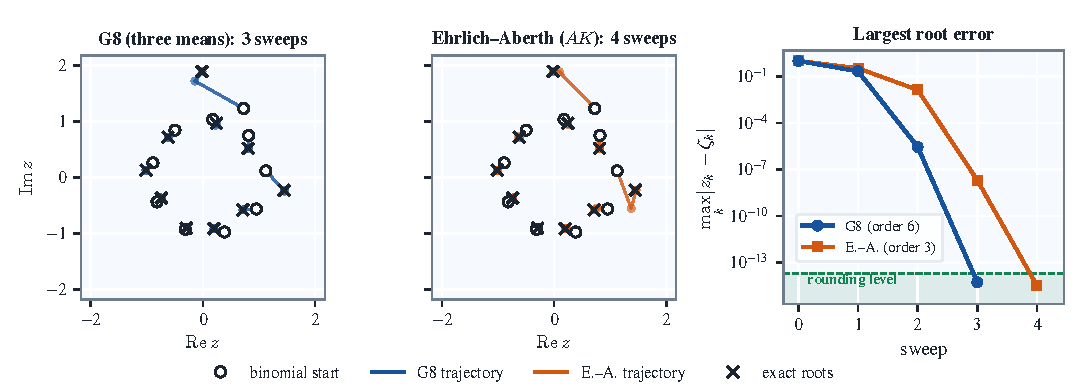
\includegraphics[width=\textwidth]{fig_paths.pdf}
\caption{One polynomial of degree 10 with complex Gaussian coefficients, from the binomial start of Section~\ref{sec:start}: trajectories after each Gauss--Seidel sweep of G8 (three means) and Ehrlich--Aberth ($AK$), and the largest root error $\max_k|z_k-\zeta_k|$. Most sweeps are spent approaching; the order-6 drop appears on the final two sweeps.}\label{fig:paths}
\end{figure}

% =========================================================================
\section{One certificate}\label{sec:cert}
Let $z_1,\dots,z_m$ be distinct and $W_k=S(z_k)\big/\bigl(c\prod_{l\ne k}(z_k-z_l)\bigr)$: the value at $z_k$ of the deflated function of Definition~\ref{def:defl} (with $y=z$), divided by $c$.

\begin{theorem}[Smith~\cite{smith}]\label{thm:smith}
Every root of $S$ lies in $\bigcup_k D(z_k,m|W_k|)$, and a connected component of this union made of $q$ discs contains exactly $q$ roots.
\end{theorem}
\begin{proof}
The polynomial $\prod_l(w-z_l)+\sum_k W_k\prod_{l\ne k}(w-z_l)$ is monic of degree $m$ and equals $S/c$ at the $m$ points $z_k$, hence everywhere:
\begin{equation}\label{eq:pf}
 \frac{S(w)}{c}=\prod_l(w-z_l)\Bigl(1+\sum_k\frac{W_k}{w-z_k}\Bigr)\qquad(w\ne z_1,\dots,z_m).
\end{equation}
It is the characteristic polynomial of $M=\operatorname{diag}(z_k)-W\mathbf{1}^\top$, whose row $k$ has centre $z_k-W_k$ and off-diagonal sum $(m-1)|W_k|$. Gershgorin's theorems~\cite{gersh} apply.
\end{proof}

The second half rests on continuity. The count used by the algorithm is obtained from Banach's fixed-point theorem alone.

\begin{theorem}[Fixed-point certificate]\label{thm:fp}
Let $\rho\ge0$ with $\rho<|z_k-z_l|$ for every $l\ne k$, and
\[
 \delta_l=|z_k-z_l|-\rho,\qquad \sigma=\sum_{l\ne k}\frac{|W_l|}{\delta_l},\qquad \tau=\sum_{l\ne k}\frac{|W_l|}{\delta_l^2}.
\]
If $\sigma<1$, $|W_k|\le\rho(1-\sigma)$ and $|W_k|\tau<(1-\sigma)^2$, the closed disc $D(z_k,\rho)$ contains exactly one root of $S$.
\end{theorem}
\begin{proof}
Let $T(w)=\sum_{l\ne k}W_l/(w-z_l)$ and $\Phi_k(w)=z_k-W_k/(1+T(w))$. On the disc, $|w-z_l|\ge\delta_l$, so $|T|\le\sigma$ and $|1+T|\ge1-\sigma>0$. By~\eqref{eq:pf}, for $w\ne z_k$ in the disc, $S(w)=0$ iff $1+W_k/(w-z_k)+T(w)=0$, i.e.\ $\Phi_k(w)=w$; and $S(z_k)=0$ iff $W_k=0$, i.e.\ $\Phi_k(z_k)=z_k$. Thus roots of $S$ in the disc are fixed points of $\Phi_k$. The disc maps into itself: $|\Phi_k(w)-z_k|\le|W_k|/(1-\sigma)\le\rho$. Since $\bigl|\frac1{w-z_l}-\frac1{w'-z_l}\bigr|\le|w-w'|/\delta_l^2$,
\[
 |\Phi_k(w)-\Phi_k(w')|=\frac{|W_k|\,|T(w)-T(w')|}{|1+T(w)|\,|1+T(w')|}
 \le\frac{|W_k|\tau}{(1-\sigma)^2}\,|w-w'|,
\]
a contraction: one fixed point exactly.
\end{proof}

\begin{corollary}\label{cor:fp}
\textup{(i)} If every $k$ satisfies Theorem~\ref{thm:fp} with a radius $\rho_k$ and the discs $D(z_k,\rho_k)$ are pairwise disjoint, $S$ has exactly one root in each disc and no other root.\\
\textup{(ii)} Let $w_l\ge|W_l|$ for every $l$, $\rho=2w_k$, and let $\sigma,\tau$ be computed with the $w_l$. If $\sigma<\frac12$ and $w_k\tau<\frac14$, Theorem~\ref{thm:fp} applies to $D(z_k,2w_k)$, and this disc is disjoint from every $D(z_l,2w_l)$, $l\ne k$.
\end{corollary}
\begin{proof}
(i) The $m$ roots found are distinct and $S$ has at most $m$ roots. (ii) $1-\sigma>\frac12$ gives $|W_k|\le w_k\le\rho(1-\sigma)$ and $|W_k|\tau<\frac14<(1-\sigma)^2$; each term of $\sigma$ is below $\frac12$, so $2w_l<|z_k-z_l|-2w_k$.
\end{proof}

The code applies (ii) then (i), replacing each gap $|z_k-z_l|-2w_k$ by a positive lower bound and testing with inflated weights $w_k(1+2^{-10})$ while returning $D(z_k,2w_k)$, so every returned disc tolerates a $2^{-10}$ rounding slack (double rounding, decimal printing) and still contains one root. Similar Lagrange-form inclusion discs go back to B\"orsch-Supan~\cite{bs} and Braess--Hadeler~\cite{bh}; Theorem~\ref{thm:fp} was chosen because its contraction proof formalises directly in Lean~4 (Section~\ref{sec:evidence}).

\begin{proposition}[Real roots]\label{prop:real}
Let $S$ be real, let discs $D_1,\dots,D_m$ contain all roots of $S$, and let $D_k$ contain exactly one root $\zeta$. Let $D$ be a disc centred on the real axis that contains $D_k$. If $D$ meets no $D_j$, $j\ne k$, then $\zeta$ is real and is the only root of $S$ in $D$. If $D_k$ does not meet the real axis, $\zeta$ is not real.
\end{proposition}
\begin{proof}
$D$ is its own mirror image, so $\bar\zeta$ is a root in $D$; every root in $D$ lies in some $D_j$, hence in $D_k$, which contains one root only.
\end{proof}

The solver returns $D=D(\operatorname{Re} z_k,\rho_k+|\operatorname{Im} z_k|)$ whenever a root is flagged real.

\begin{figure}[!htbp]\centering
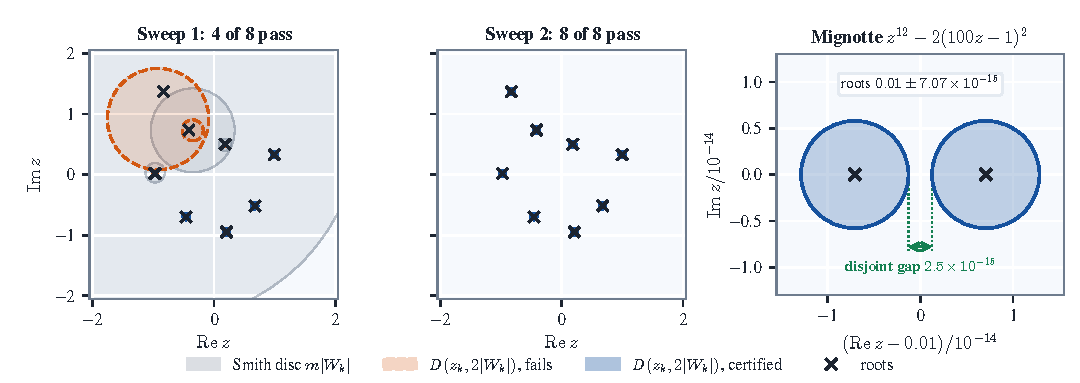
\includegraphics[width=\textwidth]{fig_discs.pdf}
\caption{The fixed-point certificate on examples. Left and centre: a complex degree-8 polynomial after Sweep~1 (4 of 8 discs pass Corollary~\ref{cor:fp}\,(ii); failing discs dashed vermilion inside translucent Smith discs) and Sweep~2 (all 8 pass, solid cobalt). Right: the two real roots of Mignotte's polynomial $z^{12}-2(100z-1)^2$, $1.41\times 10^{-14}$ apart, certified in two disjoint real discs separated by $2.5\times 10^{-15}$.}\label{fig:discs}
\end{figure}

\textbf{Arithmetic and continuation.}
The certificate needs upper bounds on $|S(z_k)|$:
\begin{itemize}
\item \emph{First certificate (double precision):} Horner's a priori bound~\cite{higham} $|S(z_k)|_{\mathrm{fl}} + \mu\bigl(\sum_j |c_j||z_k|^j + 2^{-1020}\bigr)$, $\mu=4(m+1)2^{-52}$ (doubled outside the unit disc where $1/z$ is rounded), covering subnormal underflow.
\item \emph{Values beyond double precision:} fixed-point ball evaluation with $F$ fractional bits on exact scaled coefficients (Section~\ref{sec:rust}), raising $F$ until $|P|\ge 2^r A$.
\item \emph{Products and sums:} $\prod_{l\ne k}|z_k-z_l|$ with relative margin $(8m+64)2^{-52}$; $\sigma,\tau$ with margin $(2m+16)2^{-52}$ and distances lowered by $8\cdot 2^{-52}$. A quick $O(m)$ filter checks $\sigma_k \le W/g_k$ and $\tau_k \le W/g_k^2$ from the smallest gap $g_k$ (fused with the distance-product pass) before forming the explicit $O(m^2)$ sums.
\end{itemize}
A disc is \emph{fine} if it passes Corollary~\ref{cor:fp}\,(ii), its radius is at most $\texttt{tol}\cdot|z_k|$ (default $10^{-10}$), and (for real $S$) Proposition~\ref{prop:real} decides reality---or if it has reached the floating-point grid. If any disc is not fine, the same sweep of Definition~\ref{def:sweep} continues with values beyond double precision (and, if needed, at dyadic points of higher precision).

% =========================================================================
\section{The start: dominant binomials and $O(m)$ V31 pre-polish}\label{sec:start}
Most sweeps are spent before the points enter the local basins of the roots. Write $S(z)=\sum_j a_j z^j$ and take the upper convex hull of $(j,\log|a_j|)$ (the Newton polygon). Each edge $(i,k)$ defines a binomial $a_i z^i + a_k z^k$ dominating on $|z|=|a_i/a_k|^{1/K}$, $K=k-i$, announcing $K$ roots of that modulus:
\begin{enumerate}
\item \emph{Groups.} An edge with $K=1$ is \emph{soft} if the remaining terms exceed twice the two binomial terms on its circle. Consecutive soft edges merge into one group; every other edge is its own group.
\item \emph{Shifted power.} For a group $(i,k)$ with $q(z)=a_i+\dots+a_k z^K$, its centroid is $g=-a_{k-1}/(Ka_k)$ and its starting points are $g+w^{1/K}$, $w=-q(g)/a_k$, at their true angles~\cite{c5}. For $K=1$ the point is $-a_i/a_k$.
\item \emph{Real polynomials.} Each group with $K\ge2$ is rotated by a tenth of its angular spacing to break conjugation symmetry (Section~\ref{sec:trap}).
\end{enumerate}
This extends Bini's circles~\cite{bini} with the centroid and exact angles of each group, at cost $O(m)$ per edge.

\keyidea{$O(m)$ disjoint-disc three-mean pre-polish (crate 0.30.0)}{From the Newton-polygon groups we read in $O(m)$ time a lower bound $\mathrm{sep}_k$ on each starting point's distance to all other starting points: the minimum of its own circle chord $2r\sin(\pi/K)$ and the radial gap to every other group's annulus $[||g|-r|, |g|+r]$. Setting $\mathrm{rad}_k = 0.45\,\mathrm{sep}_k$ yields pairwise-disjoint safety discs $D(z_k,\mathrm{rad}_k)$ for all $m\ge24$. Any point whose single-point three-mean step~\eqref{eq:g2} satisfies $|h_k|\le c\,\mathrm{rad}_k$ ($c=0.90$ on sparse polynomials, $c=0.25$ on dense ones) cannot collide with another iterate; its radius is updated to $\mathrm{rad}_k - |z_k^+-z_k|$ and it advances in $O(m)$ without paying for $O(m^2)$ reciprocal sums.}

On sparse polynomials (where batched Horner evaluation is $O(m)$ while reciprocal sums are $O(m^2)$) and on shifted powers, this $O(m)$ V31 pre-polish drives most or all roots straight to rounding level before a single $O(m^2)$ sweep runs (Figure~\ref{fig:start}, right).

\begin{table}[H]\centering\small
\begin{tabular}{lrr@{\qquad}lrr}
\toprule
polynomial & one circle & binomials & polynomial & one circle & binomials\\
\midrule
roots $10^k$, $k<10$ & 23 & 3 & Chebyshev 30 & 14 & 7\\
roots $2^k$, $k<20$ & 23 & 3 & Mignotte, degree 12 & 16 & 9\\
coefficients from $10^{-8}$ to $10^{8}$ & 23 & 2 & $\exp$ truncated, degree 40 & 15 & 9\\
$(z^{10}-1)(z^{10}-10^{20})$ & 20 & 2 & $(z-3)^{12}-5$ & 2 & 5\\
Wilkinson 20 & $9+17$ & $12+5$ & Wilkinson 10 & 7 & 9\\
\bottomrule
\end{tabular}
\caption{Sweeps in double precision (for Wilkinson 20: plus exact-value sweeps). Of 21 test families, the dominant-binomial start needs fewer sweeps in 12 and more in 5: a single circle remains better when all roots cluster away from the origin. On random polynomials see Table~\ref{tab:random}.}\label{tab:start}
\end{table}

\begin{figure}[!htbp]\centering
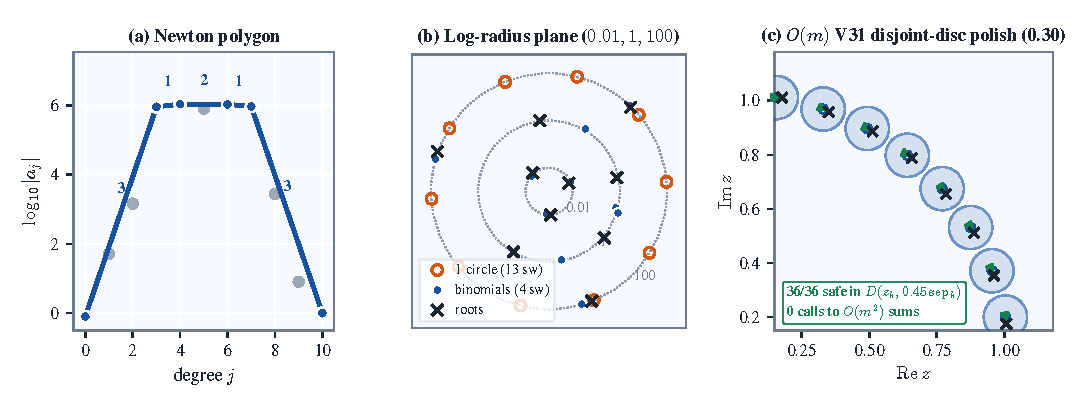
\includegraphics[width=\textwidth]{fig_start_v31.pdf}
\caption{Dominant binomials and $O(m)$ V31 pre-polish. (a)~Upper convex hull (Newton polygon) of a degree-10 polynomial with roots at three scales ($0.01, 1, 100$); numbers give group multiplicities. (b)~Logarithmic-radius plane: binomials converge in 4 sweeps against 13 from one circle. (c)~Disjoint-disc $O(m)$ V31 pre-polish (crate 0.30.0) on the sparse degree-36 polynomial $3z^{36}-0.35z^{23}+0.28z^{11}-7$: all 36 single-point three-mean steps stay strictly inside their pairwise-disjoint discs $D(z_k, 0.45\,\mathrm{sep}_k)$ and land on the roots with zero calls to $O(m^2)$ sums.}\label{fig:start}
\end{figure}

% =========================================================================
\section{The algorithm}\label{sec:algo}
\begin{enumerate}
\item \emph{Zero deflation and square-free decomposition:} remove $z^k$ exactly (multiplicity $k$, radius $0$); test square-freeness modulo primes; if needed compute $P=c\prod_k S_k^k$ exactly via modular GCDs with CRT reconstruction, accepted only on exact division~\cite{g5,g6}.
\item \emph{Start:} for each factor $S$ of degree $m$, form the dominant-binomial start with safety radii $\mathrm{rad}_k$ (Section~\ref{sec:start}); if the coefficients span beyond double precision or fail \texttt{Poly::fits}, start directly from exact-coefficient binomials.
\item \emph{Double-precision phase:} run the $O(m)$ disjoint-disc V31 pre-polish when applicable, then Gauss--Seidel sweeps of Definition~\ref{def:sweep} (quantising points to 53-bit moduli as they move, skipping settled points) until residuals reach rounding level (at most $100+10m$ sweeps).
\item \emph{Exact-value and multiprecision continuation:} evaluate the certificate of Section~\ref{sec:cert}. While any disc is not fine, sweep with fixed-point ball evaluations (up to $1+4$ Gauss--Seidel passes per evaluation, Section~\ref{sec:rust}) and cluster moves (Section~\ref{sec:cluster}), keeping the best certified state (at most $30+m$ certificates). When tolerance or separation requires more than 53 bits, continue at dyadic points up to 4096 bits, followed by local variable \texttt{zoom} if roots remain below $2^{-500}$.
\item \emph{Output:} if every disc passes Corollary~\ref{cor:fp}, return the $m$ disjoint discs $D(z_k,2w_k)$, one root in each; otherwise return one enclosing disc per Smith component with its root count. Each disc carries its exact multiplicity $k$ and, for real $P$, the reality flag of Proposition~\ref{prop:real}.
\end{enumerate}

\begin{theorem}\label{thm:g8}
The algorithm stops. If the floating-point and ball bounds (of $|S(z_k)|$, of the products, and of $\sigma,\tau$) are valid and the approximations of each factor are distinct, every output disc with multiplicity $k$ and count $q$ contains exactly $q$ distinct roots of $P$, each of multiplicity $k$; the counts weighted by the multiplicities add up to $\deg P$; a root flagged real is real.
\end{theorem}
\begin{proof}
All loops are bounded. The claims follow from Corollary~\ref{cor:fp} (or Theorem~\ref{thm:smith} on unresolved components), Proposition~\ref{prop:real}, and the exact square-free decomposition.
\end{proof}

% =========================================================================
\section{A trap for real polynomials}\label{sec:trap}
\begin{proposition}\label{prop:trap}
Let $S$ be real with two real roots $x\pm d$, let two approximations be $x\pm iy$ and let the others sit on the other roots. One Ehrlich--Aberth step sends $y=d\tan\theta$ to $d\tan3\theta$ and leaves $x$ unchanged. More generally, for $x\pm w$ with any complex $w$, the step sends $w$ to $w^+=w\,\dfrac{w^2+3d^2}{3w^2+d^2}$, and
\[
 \frac{w^+-d}{w^++d}=\Bigl(\frac{w-d}{w+d}\Bigr)^{3}.
\]
\end{proposition}
\begin{proof}
For $x+w$: $A=\frac1{w-d}+\frac1{w+d}-\frac1{2w}=\frac{3w^2+d^2}{2w\,(w^2-d^2)}$, so $w-1/A=w\,\frac{w^2+3d^2}{3w^2+d^2}$ and $w^+\mp d=(w\mp d)^3/(3w^2+d^2)$. For $w=iy$, $(w-d)/(w+d)$ lies on the unit circle with argument $\pi-2\theta$: the step cubes it and triples the angle.
\end{proof}
In exact arithmetic any sweep commuting with conjugation traps a conjugate pair on the unit circle of $(w-d)/(w+d)$ forever. The asymmetric rotation of Section~\ref{sec:start} avoids this in double precision; in exact-value sweeps, if rounded coefficients momentarily create a conjugate pair, rounding of the sums breaks the symmetry.

\begin{remark}[The real axis, where the support matters]\label{rem:axis}
For a real polynomial, Ehrlich--Aberth maps $\R^m$ into $\R^m$: real approximations can never reach a complex conjugate pair. The square roots of $q_M(t)$ naturally leave the real axis whenever the cursor is negative. With the binomial start (which places $K=1$ groups on $\R$), $AK$ fails on 1 of 400 random real degree-5 polynomials (150 sweeps, two clusters), while the three means solve all 400.
\end{remark}

\begin{figure}[!htbp]\centering
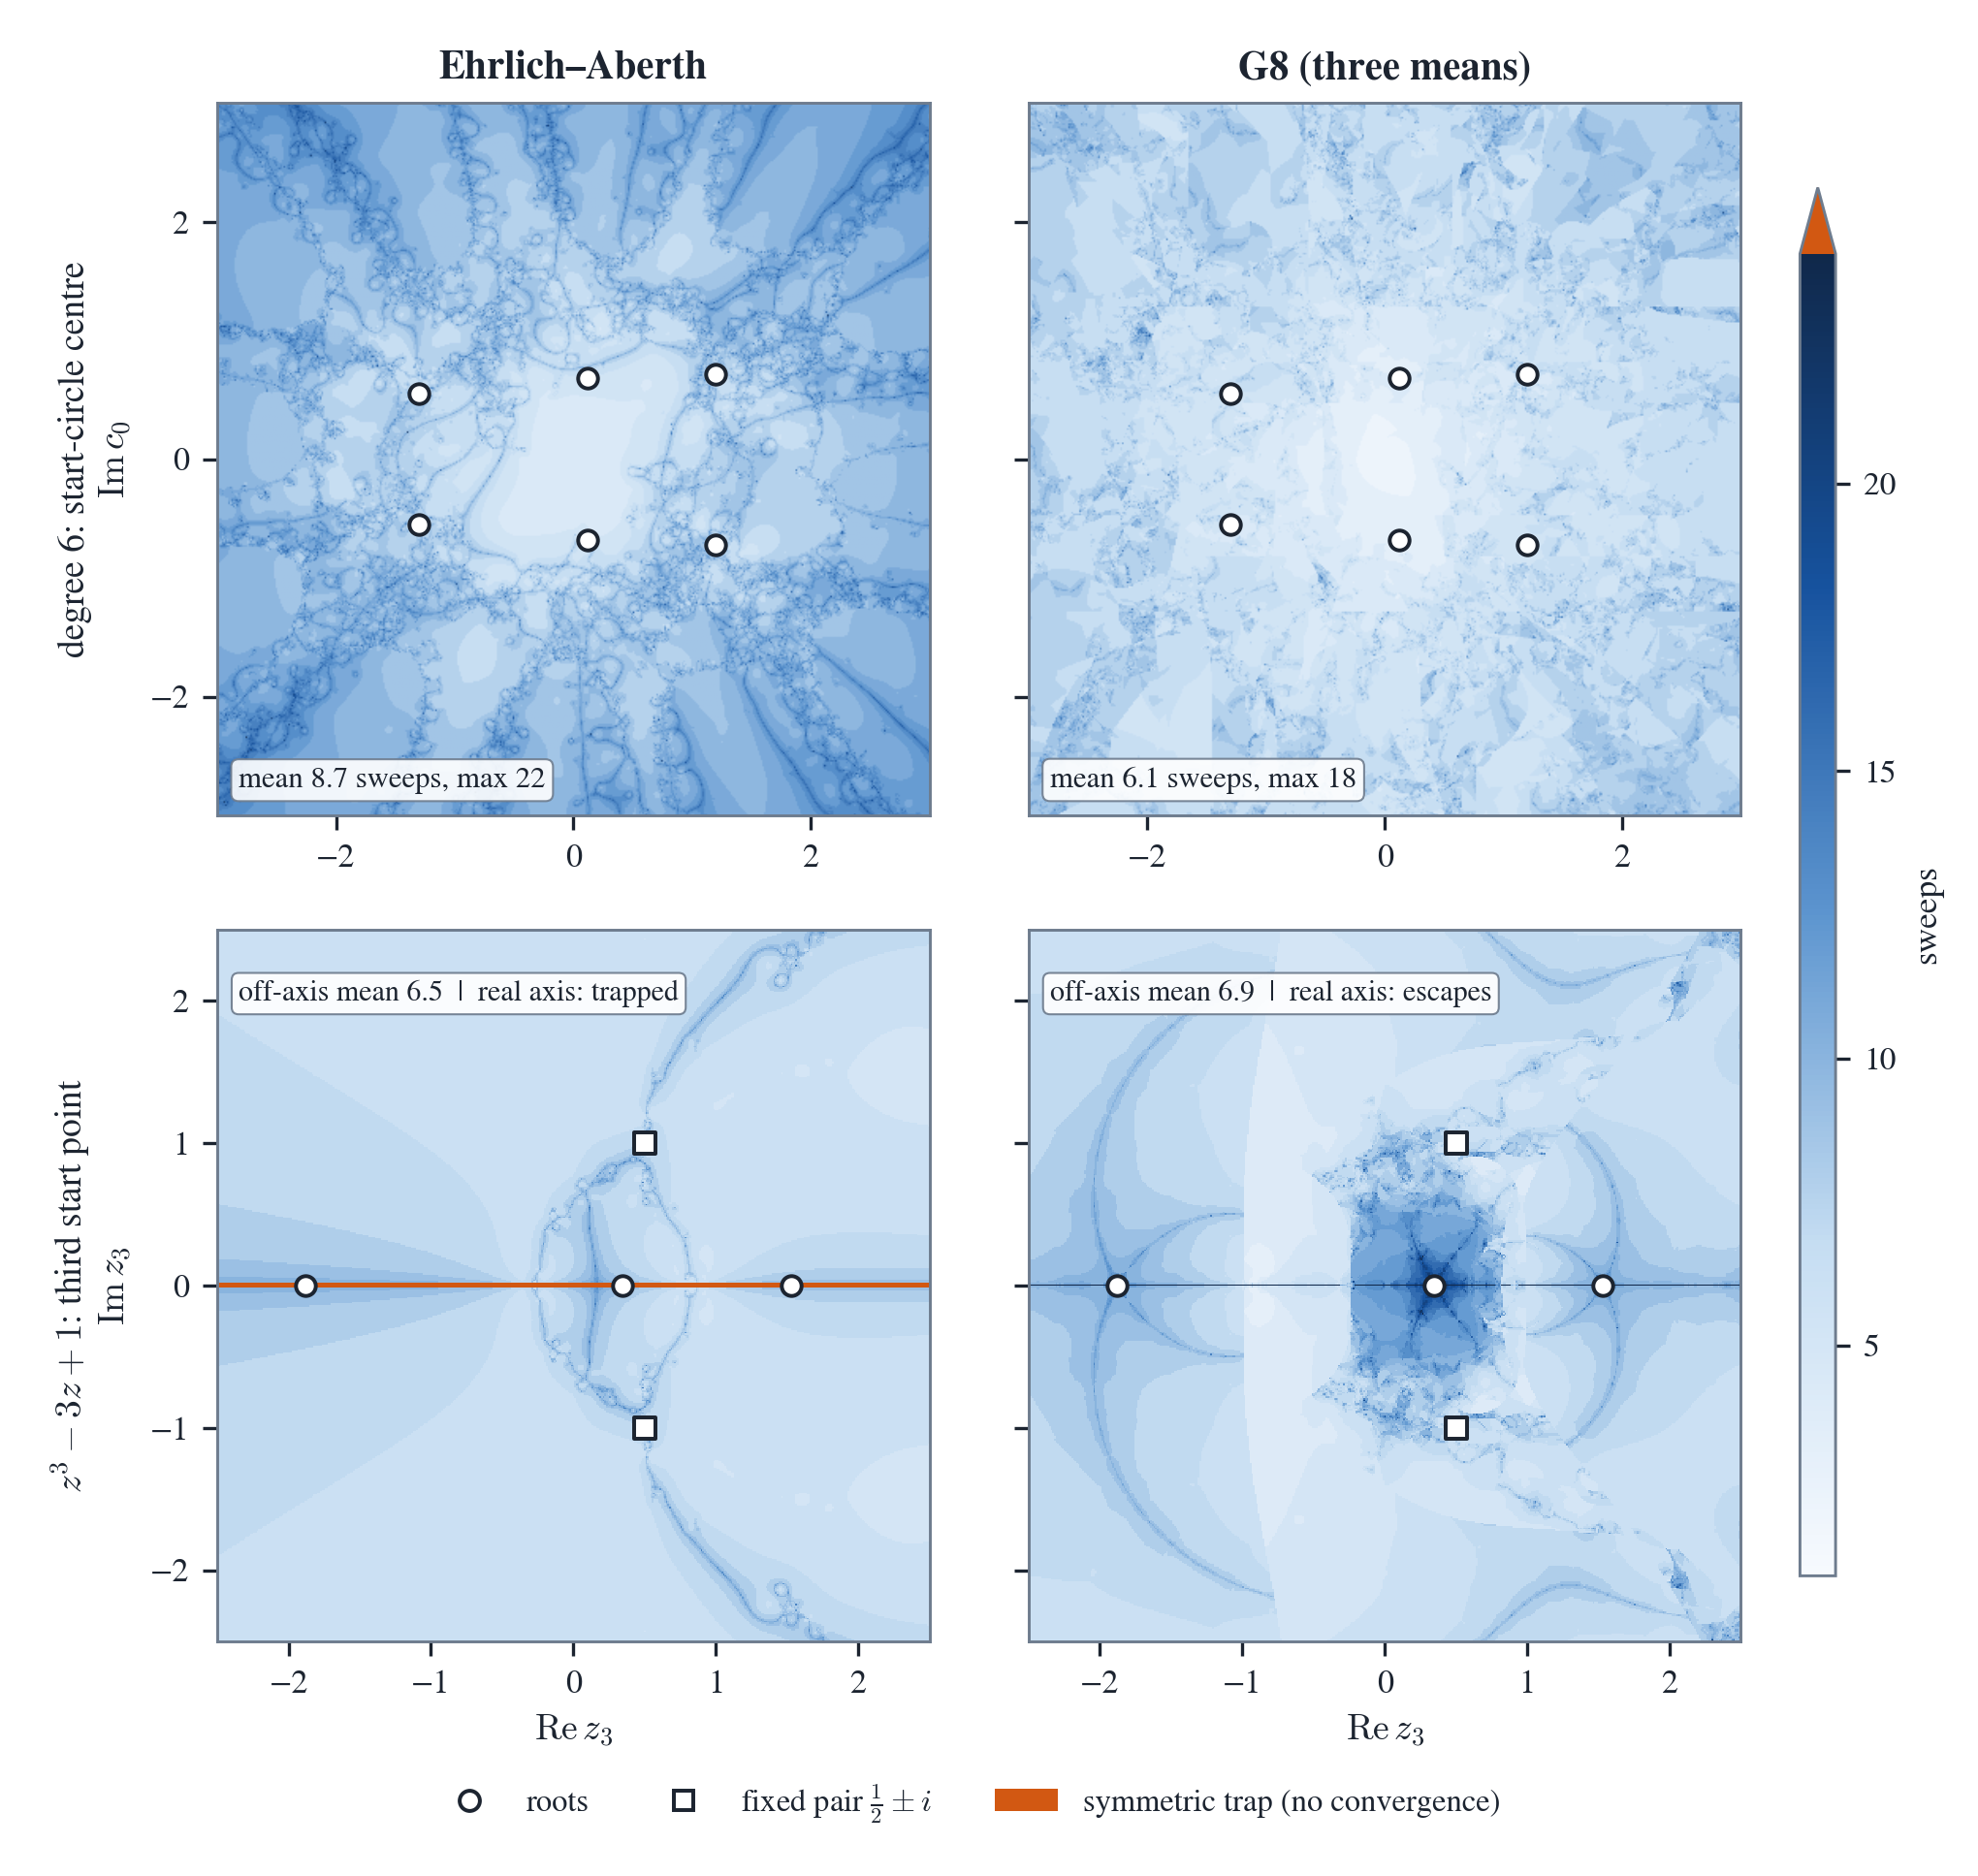
\includegraphics[width=0.95\textwidth]{fig_sweeps.png}
\caption{Number of sweeps as a function of the start on two 2D slices ($451\times 451$ grid). \textbf{Top:} a real degree-6 polynomial with three conjugate pairs; six points start on a circle of radius $1.3$ whose centre $c_0$ moves over $[-3,3]^2$ (G8 mean 6.1 sweeps vs.\ Ehrlich--Aberth 8.7). \textbf{Bottom:} $z^3-3z+1$ (three real roots) with two points fixed at $\frac12\pm i$ and the third varying over $[-2.5,2.5]^2$. On the real axis the start is symmetric (Proposition~\ref{prop:trap}): Ehrlich--Aberth remains trapped forever across the entire axis (vermilion line), whereas G8 loses exact symmetry at rounding level and converges from every point of the window.}\label{fig:sweeps}
\end{figure}

% =========================================================================
\section{Prototype measurements}\label{sec:meas}
We retain the baseline Python prototype measurements (\texttt{verify\_g8.py}) to isolate the mathematical effect of the support and start independently of compiled low-level optimisations (Section~\ref{sec:rust}). On 2600 Gaussian random polynomials of degree 5 to 160, every root was isolated and certified in double precision (no exact-value sweep needed; median largest relative radius $2\cdot10^{-14}$ at degree~5 to $6\cdot10^{-13}$ at degree~160).

\begin{table}[H]\centering\small\setlength{\tabcolsep}{4.5pt}
\begin{tabular}{lr@{\quad}rrr@{\qquad}rrr}
\toprule
 & & \multicolumn{3}{c}{complex coefficients} & \multicolumn{3}{c}{real coefficients}\\
degree & number & G8 & G8, one circle & E.--A. & G8 & G8, one circle & E.--A.\\
\midrule
5 & 400 & 2.54 (7) & 3.45 (8) & 3.91 (7) & 2.69 (8) & 4.04 (8) & 4.56 (149)\\
10 & 400 & 3.35 (8) & 4.32 (9) & 4.96 (11) & 3.51 (9) & 4.81 (12) & 5.35 (18)\\
20 & 300 & 4.29 (9) & 5.22 (14) & 6.26 (12) & 4.51 (11) & 5.85 (17) & 6.69 (14)\\
40 & 150 & 5.35 (11) & 6.09 (14) & 7.89 (13) & 5.72 (10) & 6.93 (21) & 8.42 (12)\\
80 & 40 & 6.72 (10) & 7.40 (10) & 9.03 (12) & 6.90 (12) & 7.92 (12) & 10.20 (13)\\
160 & 10 & 7.10 (9) & 8.40 (10) & 10.40 (15) & 8.00 (10) & 9.30 (15) & 11.00 (18)\\
\bottomrule
\end{tabular}
\caption{Mean sweeps in the Python prototype (maximum in brackets; 2600 polynomials). ``E.--A.'': Ehrlich--Aberth from the same binomial start. G8 uses 26 to 41\,\% fewer sweeps than Ehrlich--Aberth, and 9 to 33\,\% fewer than from one circle.}\label{tab:random}
\end{table}

\begin{table}[H]\centering\small
\begin{tabular}{llrrr}
\toprule
support on $F_k$ & announced by & all roots found & mean sweeps & maximum\\
\midrule
$AK$ (Ehrlich--Aberth) & nothing & 300 & 6.54 & 12\\
line $AD$ & nothing & 270 & 5.60 & 11\\
conic & nothing & 300 & 6.65 & 23\\
three means & nothing & 300 & 6.42 & 21\\
$AK$ & three means & 300 & 5.82 & 12\\
three means & line $AD$ (Halley) & 300 & 4.63 & 9\\
conic & conic & 300 & 4.38 & 10\\
three means & three means & 300 & 4.34 & 9\\
\bottomrule
\end{tabular}
\caption{Support comparison on 300 random polynomials (degrees 10, 20, 40, half real). The sweep reduction comes from applying a second-order support twice; the three means and the conic agree within 1\,\%.}\label{tab:support_py}
\end{table}

% =========================================================================
\section{The Rust implementation: \texttt{pandroots} 0.1.0 to 0.30.0}\label{sec:rust}
The crate \texttt{pandroots} (\url{https://crates.io/crates/pandroots}, version 0.30.0, zero \texttt{unsafe} code, about 6\,500 lines excluding tests, using \texttt{num-bigint} outside the fixed-width limb kernels) implements the complete chain in double precision (\texttt{all\_roots}, \texttt{all\_roots\_exact}) and arbitrary precision (\texttt{all\_roots\_precise}, \texttt{all\_roots\_exact\_precise}, tolerances down to $10^{-280}$, points up to 4096 bits plus local zoom).

\subsection{Foundations (versions 0.1.0 to 0.12.0)}
Revision~9 documented the first twelve releases in detail; we summarise the milestones that remain in 0.30.0:
\begin{itemize}
\item \emph{Gauss--Seidel order and overflow-free evaluation (0.1.0--0.3.0):} outside the unit disc $S'/S$ and $S''/S$ are evaluated through the reversed polynomial $w^m S(1/w)$; exact power-of-two variable and coefficient scaling ($z=2^s u$ minimising coefficient binary spread); underflow-safe Horner bound $\mu(\sum|c_j||z|^j+2^{-1020})$; coincident-point nudging.
\item \emph{Multiprecision continuation (0.4.0--0.5.0):} with $N=S/S'$, $\beta=SS''/S'^2$, $u=s_1 N$, $v=s_2 N^2$, the step~\eqref{eq:step} with $p=m$ rewrites as
\begin{equation}\label{eq:precise}
\begin{aligned}
 (1-u)^2(t_k-1)&=\frac{m(2u-u^2-\beta-v)}{m-1}, &
 \kappa&=\frac{(m-1)(q(t_k)-1)}{m},\\
 z_k^+&=z_k-\frac{N}{1+w}, &
 w&=\kappa-u-u\kappa.
\end{aligned}
\end{equation}
By default, $N$ is a multiprecision quotient from the ball evaluation while only the correction $w$ is formed in double precision (doubling correct digits every sweep); \texttt{Options::full\_order} evaluates $s_1,s_2$ and $q_M$ in multiprecision (\texttt{three\_fx}) to retain order~6.
\item \emph{Zero deflation, modular square-free decomposition, fixed-width arithmetic, scaled variables, and dual start (0.6.0--0.12.0):} $P=z^k Q$ deflation; Yun's GCDs via primes $p\equiv 1\pmod4$ and CRT verified by exact division; fixed-width limb Horner buffers; per-point bit memory; scaled variable $T(t)=S(2^e t)$ for short multipliers far from the unit circle; exact-coefficient binomial start for extreme scales; 24-point median Smith-radius comparison against \texttt{Start::Edges} when double precision leaves $\ge 25\,\%$ of points uncertified.
\end{itemize}
In the external MPSolve~3.2.3 comparison~\cite{mpsolve} reported in revision~9 (462 polynomials at 10 digits and 100 at 14, 30 and 80 digits), \texttt{pandroots} 0.5.0--0.10.1 passed 462/462 at 10 digits and 100/100 at 14, 30 and 80 digits (geometric mean speed ratio of MPSolve over the crate: 4.06 at 10 digits, 2.03 at 30 digits, 3.14 at 80 digits), with MPSolve remaining ahead on 5-root clusters, monomials, and slightly on Wilkinson polynomials.

\subsection{Evolution from 0.13.0 to 0.30.0}
Eighteen releases since revision~9 widened the corpus from 10\,000 to 100\,000 polynomials and accelerated every phase while keeping the single-path three-mean architecture intact:
\begin{itemize}
\item \emph{Double-precision and sparse kernels (0.13.0, 0.27.0, 0.29.0, 0.30.0):} points are quantised as they move so the final sweep evaluation serves the certificate directly; settled points skip re-evaluation (\texttt{Poly::ev\_some}); dense Horner processes 4-point register blocks with portable FMA (\texttt{f64::mul\_add}), strictly tightening Higham's rounding bound while preserving single-point bit identity; reciprocal sums use 8 FMA lanes; sparse polynomials ($\ge 12$ zeros per nonzero) jump zero runs with 4-wide batched evaluation sharing a single $x^{2^b}, |x|^{2^b}$ power table (\texttt{sparse\_eval\_batch}, bit-for-bit identical to scalar Horner); the $O(m)$ disjoint-disc V31 pre-polish (Section~\ref{sec:start}) eliminates $O(m^2)$ sweeps on sparse and shifted-power polynomials.
\item \emph{Certificate and distance-product fusion (0.13.0, 0.18.0, 0.29.0, 0.30.0):} Smith denominator products are cached across certificate passes and fused with the smallest-gap scan in a 4$\times$4 upper-triangular tiled kernel (\texttt{products\_and\_min\_sq}) with hoisted range/finiteness checks every 48 columns and branch-free \texttt{frexp\_normal}; an $O(m)$ overlap check ($2\max_k r_k < \min_k\sqrt{\mathrm{min\_sq}_k}$) skips $O(m^2)$ distance-matrix and component construction whenever no discs overlap.
\item \emph{Two's-complement fused Horner and zero-allocation ball evaluation (0.14.0, 0.17.0, 0.29.0, 0.30.0):} short-multiplier Horner works in two's complement with cached limb tables (half-size for real polynomials), unsigned \texttt{u128} low-limb multiplies with hoisted signs, tight stack arrays for widths $N=3\dots16$, and fused 3-chain loops (\texttt{horner3\_tc\_fused}, \texttt{horner3\_tc\_real\_fused} for $N=3\dots6$) executing all carry chains in parallel. Version 0.30.0 eliminates \texttt{BigInt} allocations on the exact-stage hot path via direct \texttt{Short::from\_zp\_shifted}, \texttt{tc\_to\_float}, and \texttt{horner\_floats\_short} (and \texttt{horner3\_short\_zp} when multiprecision \texttt{parts} are requested), and evaluates $S(z_k)$ value-only (\texttt{horner0}, $3\times$ faster) first on points expected to certify when $\texttt{tol}\ge10^{-12}$.
\item \emph{Multi-pass exact sweeps (0.24.0, 0.30.0):} in exact-value sweeps, an evaluation costs hundreds of bits per coefficient while double-precision sums are cheap. \texttt{rectangle\_step\_again} performs additional Gauss--Seidel passes over the sums from the same exact values of $S,S',S''$ (2 extra passes in 0.24.0; up to 4 early-stopping passes in 0.30.0). The roots are a fixed point of every pass (\texttt{SecondPass.lean}, Section~\ref{sec:evidence}), cutting exact sweeps by 10--18\,\% on Wilkinson, orthogonal, powers, and Mignotte families.
\item \emph{C5 slit-plane branch, spherical damping, wide scales, and cluster/zoom completeness (0.15.0--0.29.0):} opt-in spherical great-circle damping (\texttt{riemann-iterations}, 0.15.0--0.16.0); bounded integer dyadic verifier \texttt{verify\_dyadic\_discs} extracted with Aeneas (0.19.0--0.21.0); wide-scale detection \texttt{Poly::fits} (0.23.0); quadratic step at $S'=0$ (0.25.0); local variable \texttt{zoom} beyond $2^{-500}$ (0.26.0); circle retry for whole-factor clusters (0.28.0); C5 slit-plane branch of $q_M(t)$ and outermost-member cluster-cursor fallback (0.29.0); Barrett modular GCDs in \texttt{sqfree} (0.30.0).
\end{itemize}

\subsection{Measurements of \texttt{pandroots 0.30.0}}

\textbf{100\,000-polynomial corpus} (5\,060\,069 roots across 16 families, degrees up to 2000; 36\,000 polynomials built from prescribed rational roots checked against exact rational oracles; Apple~M5, 1 thread, versions alternating per polynomial in a single binary, \texttt{Options::default()}). Table~\ref{tab:100k} reports the complete family breakdown from 0.28.0 through 0.29.0 to 0.30.0.

\begin{table}[H]\centering\small\setlength{\tabcolsep}{4.2pt}
\begin{tabular}{lrrrrrrrrr}
\toprule
family & polys & roots & 0.28.0 (s) & 0.29.0 (s) & 0.30.0 (s) & $\frac{0.29}{0.30}$ & $\frac{0.28}{0.30}$ & \texttt{swp\_x} & \texttt{crt\_x}\\
\midrule
\texttt{sparse}       &  5\,000 & 2\,173\,370 & 9.161 & 4.536 & \textbf{3.041} & 1.49$\times$ & \textbf{3.01$\times$} & 1.46$\times$ & 1.90$\times$\\
\texttt{dense\_large} &  1\,200 &    711\,360 & 5.969 & 3.228 & \textbf{3.085} & 1.05$\times$ & \textbf{1.93$\times$} & 1.00$\times$ & 1.88$\times$\\
\texttt{orthogonal}   &  2\,500 &    119\,600 & 4.060 & 2.734 & \textbf{2.365} & 1.16$\times$ & \textbf{1.72$\times$} & 0.96$\times$ & 1.17$\times$\\
\texttt{powers}       &  5\,000 &    265\,766 & 3.195 & 2.187 & \textbf{1.796} & 1.22$\times$ & \textbf{1.78$\times$} & 1.25$\times$ & 1.22$\times$\\
\texttt{cluster}      & 12\,000 &     91\,193 & 2.091 & 1.658 & \textbf{1.600} & 1.04$\times$ & \textbf{1.31$\times$} & 0.98$\times$ & 1.04$\times$\\
\texttt{wilkinson}    &  2\,500 &     81\,255 & 2.226 & 1.534 & \textbf{1.261} & 1.22$\times$ & \textbf{1.77$\times$} & 0.97$\times$ & 1.24$\times$\\
\texttt{multiplicity} &  8\,000 &    124\,631 & 1.320 & 0.773 & \textbf{0.773} & 1.00$\times$ & \textbf{1.71$\times$} & 0.95$\times$ & 1.03$\times$\\
\texttt{mignotte}     &  3\,000 &    131\,618 & 0.861 & 0.695 & \textbf{0.636} & 1.09$\times$ & \textbf{1.35$\times$} & 1.18$\times$ & 1.09$\times$\\
\texttt{special}      &  2\,000 &    113\,158 & 1.015 & 0.725 & \textbf{0.626} & 1.16$\times$ & \textbf{1.62$\times$} & 0.98$\times$ & 1.19$\times$\\
\texttt{dense}        & 28\,800 &    753\,971 & 0.785 & 0.577 & \textbf{0.572} & 1.01$\times$ & \textbf{1.37$\times$} & 0.99$\times$ & 1.27$\times$\\
\texttt{products}     &  2\,500 &     78\,750 & 0.340 & 0.260 & \textbf{0.258} & 1.01$\times$ & \textbf{1.32$\times$} & 0.94$\times$ & 1.34$\times$\\
\texttt{roots}        & 10\,000 &    126\,478 & 0.290 & 0.229 & \textbf{0.204} & 1.12$\times$ & \textbf{1.42$\times$} & 0.97$\times$ & 1.31$\times$\\
\texttt{laws}         & 10\,000 &    207\,168 & 0.175 & 0.133 & \textbf{0.131} & 1.02$\times$ & \textbf{1.34$\times$} & 0.98$\times$ & 1.23$\times$\\
\texttt{zero\_roots}  &  2\,000 &     43\,588 & 0.105 & 0.090 & \textbf{0.090} & 1.00$\times$ & \textbf{1.17$\times$} & 1.00$\times$ & 1.05$\times$\\
\texttt{scales}       &  2\,500 &     24\,438 & 0.098 & 0.053 & \textbf{0.053} & 1.00$\times$ & \textbf{1.85$\times$} & 0.98$\times$ & 1.01$\times$\\
\texttt{edges}        &  3\,000 &     13\,725 & 0.015 & 0.010 & \textbf{0.010} & 1.00$\times$ & \textbf{1.50$\times$} & 1.00$\times$ & 1.04$\times$\\
\midrule
\textbf{TOTAL} & \textbf{100\,000} & \textbf{5\,060\,069} & \textbf{30.261} & \textbf{19.422} & \textbf{16.499} & \textbf{1.18$\times$} & \textbf{1.83$\times$} & \textbf{1.17$\times$} & \textbf{1.22$\times$}\\
\bottomrule
\end{tabular}
\caption{100\,000-polynomial A/B benchmark (Apple~M5, 1 thread, \texttt{Options::default()}). The 0.29.0 vs.\ 0.30.0 columns come from one alternating paired run; 0.28.0 is from the paired 0.28.0 vs.\ 0.29.0 run on the same corpus and machine (where 0.29.0 took 19.276\,s). Every version certifies 100\,000/100\,000 polynomials completely and passes all 36\,000/36\,000 exact rational oracles (0 failed). Isolation within $10^{-10}$ reaches 92\,043 in 0.30.0 (92\,037 in 0.29.0, $+6$ net); the remaining 7\,957 are clusters and Mignotte pairs finer than the double-precision grid. Columns \texttt{swp\_x} and \texttt{crt\_x} show the 0.29.0$\to$0.30.0 speedups of double-precision sweeps and certification respectively.}\label{tab:100k}
\end{table}

\textbf{Stratified \texttt{precise} mode.}
On a stratified subset of the hardest families (\texttt{mignotte}, \texttt{cluster}, \texttt{wilkinson}, \texttt{orthogonal}, \texttt{special}, \texttt{scales}, \texttt{dense}) via \texttt{all\_roots\_precise}/\texttt{all\_roots\_exact\_precise}:
\begin{itemize}
\item At $\texttt{tol}=10^{-10}$ ($n=1036$): $3.592\,\mathrm{s}\ (0.28.0) \to 3.248\,\mathrm{s}\ (0.29.0) \to \mathbf{3.051\,\mathrm{s}}\ (0.30.0)$, \textbf{1036/1036} complete and isolated (against 1035/1036 in 0.29.0; 129 zooms).
\item At $\texttt{tol}=10^{-30}$ ($n=518$): $2.413\,\mathrm{s}\ (0.28.0) \to 2.238\,\mathrm{s}\ (0.29.0) \to \mathbf{2.158\,\mathrm{s}}\ (0.30.0)$, \textbf{518/518} complete and isolated (94 zooms).
\end{itemize}

\textbf{High-precision single calls} (Table~\ref{tab:hp}, comparing default vs.\ \texttt{full\_order} in \texttt{pandroots 0.30.0}, plus local zoom beyond $2^{-500}$).

\begin{table}[H]\centering\small
\begin{tabular}{lrrr}
\toprule
polynomial & digits & default (ms, sweeps) & \texttt{full\_order} (ms, sweeps)\\
\midrule
dense, integer coefficients, degree 60  &  30 &   1.79 (1) &   1.96 (1)\\
                                        &  80 &   4.08 (2) &   7.63 (2)\\
                                        & 280 &  15.86 (4) &  19.78 (3)\\
dense, integer coefficients, degree 160 &  30 &  10.99 (1) &  10.79 (1)\\
                                        &  80 &  36.40 (3) &  50.89 (2)\\
                                        & 280 & 111.78 (4) & 139.45 (3)\\
dense, integer coefficients, degree 320 &  30 &  56.92 (1) &  54.96 (1)\\
                                        &  80 & 122.54 (2) & 197.30 (2)\\
                                        & 280 & 452.23 (4) & 538.45 (3)\\
$z^{1000}-1$                            &  80 &  40.45 (2) & 683.67 (2)\\
                                        & 280 & 102.04 (4) & 1238.37 (3)\\
Wilkinson 30                            &  80 &   0.40 (0) &   0.50 (0)\\
Mignotte $z^{12}-2(10^8 z-1)^2$         &  30 &   0.24 (6) &   0.34 (6)\\
$(z-1)(2^{600}z-2^{600}-1)$ (zoom)      &  10 &   0.48 (1 zoom) & ---\\
$(z-1)(2^{4000}z-2^{4000}-1)$ (zoom)    &  10 &   0.49 (1 zoom) & ---\\
\bottomrule
\end{tabular}
\caption{\texttt{pandroots 0.30.0} single-call high-precision times (milliseconds, best of three, Apple~M5, 1 thread). Compared with 0.12.0 in revision~9: dense degree~60 drops from 3.3/6.1/22.6\,ms to 1.79/4.08/15.86\,ms; $z^{1000}-1$ at 80/280 digits drops from 89.2/179\,ms to 40.45/102.04\,ms; Wilkinson~30 at 80 digits drops from 2.6\,ms to 0.40\,ms; Mignotte at 30 digits drops from 0.50\,ms (9 sweeps) to 0.24\,ms (6 sweeps). The $2^{-600}$ and $2^{-4000}$ pairs are each isolated into two disjoint certified discs in under 0.5\,ms via one local zoom.}\label{tab:hp}
\end{table}

\textbf{Double precision vs.\ \texttt{numpy.roots} / LAPACK and support cost} (Tables~\ref{tab:time} and~\ref{tab:sup_rust}, Figure~\ref{fig:bench}).

\begin{table}[H]\centering\small\setlength{\tabcolsep}{4.3pt}
\begin{tabular}{lrrrr@{\qquad}rrrr}
\toprule
 & \multicolumn{4}{c}{complex coefficients} & \multicolumn{4}{c}{real coefficients}\\
degree & sweeps & \texttt{pandroots} & \texttt{numpy.roots} & LAPACK & sweeps & \texttt{pandroots} & \texttt{numpy.roots} & LAPACK\\
\midrule
5   & 2.44 &   2.2 &    13.0 &     8.7 & 2.54 &   2.4 &    10.2 &     5.9\\
10  & 3.16 &   4.3 &    27.6 &    23.5 & 3.22 &   4.4 &    14.6 &    10.3\\
20  & 3.74 &   9.4 &    95.6 &    88.6 & 3.98 &   9.2 &    34.0 &    29.2\\
40  & 4.61 &  21.0 &   402.2 &   389.3 & 4.91 &  22.2 &   116.7 &   107.4\\
80  & 5.20 &  55.1 &  4147.1 &  4125.3 & 5.97 &  58.0 &  1084.0 &  1069.7\\
160 & 6.64 & 168.5 & 20051.7 & 19952.3 & 7.40 & 173.0 &  5405.0 &  5679.2\\
320 & 6.70 & 553.0 & 112092.2 & 117329.3 & 8.20 & 577.5 & 27914.3 & 26960.5\\
\bottomrule
\end{tabular}
\caption{Double-precision time ($\mu$s per polynomial, best of five runs, 1 thread, Apple~M5). \texttt{pandroots 0.30.0} returns certified disjoint discs and is 3.2$\times$ faster than 0.12.0 at degree~320 (553\,$\mu$s against 1795\,$\mu$s), reaching \textbf{203$\times$} faster than \texttt{numpy.roots}/LAPACK (complex) and \textbf{48$\times$} faster (real) at degree~320.}\label{tab:time}
\end{table}

\begin{table}[H]\centering\small
\begin{tabular}{llrrr}
\toprule
support on $F_k$ & neighbours announced by & degree 20 & degree 80 & degree 320\\
\midrule
$AK$ (Ehrlich--Aberth) & nothing & 7.3 (5.66) & 55.0 (7.84) & 743.1 (9.50)\\
$AK$ & their own step $AK$ & 7.2 (5.44) & 57.1 (7.44) & 742.4 (9.90)\\
$AK$ & three means & 7.8 (4.62) & 55.4 (6.92) & 616.1 (9.00)\\
three means & step $AK$ & 8.5 (4.39) & 53.7 (6.20) & 569.3 (8.50)\\
three means & three means (G8) & 8.8 (3.75) & 54.5 (5.32) & \textbf{554.4 (6.80)}\\
\bottomrule
\end{tabular}
\caption{Support comparison inside \texttt{pandroots 0.30.0} ($\mu$s per polynomial, mean sweeps in brackets, complex Gaussian coefficients, Apple~M5). Unlike 0.12.0 where Ehrlich--Aberth and G8 tied in wall-clock time at degree~320, FMA-vectorised Horner blocks and 8-lane sums in 0.30.0 amortise $S''$ and $s_2$ so that the three-mean rectangle now wins in wall-clock time as well as sweep count at degree~320 (554\,$\mu$s vs.\ 743\,$\mu$s, 1.34$\times$ faster), ties at degree~80, and trails slightly at degree~20 (8.8 vs.\ 7.3\,$\mu$s).}\label{tab:sup_rust}
\end{table}

\begin{figure}[!htbp]\centering
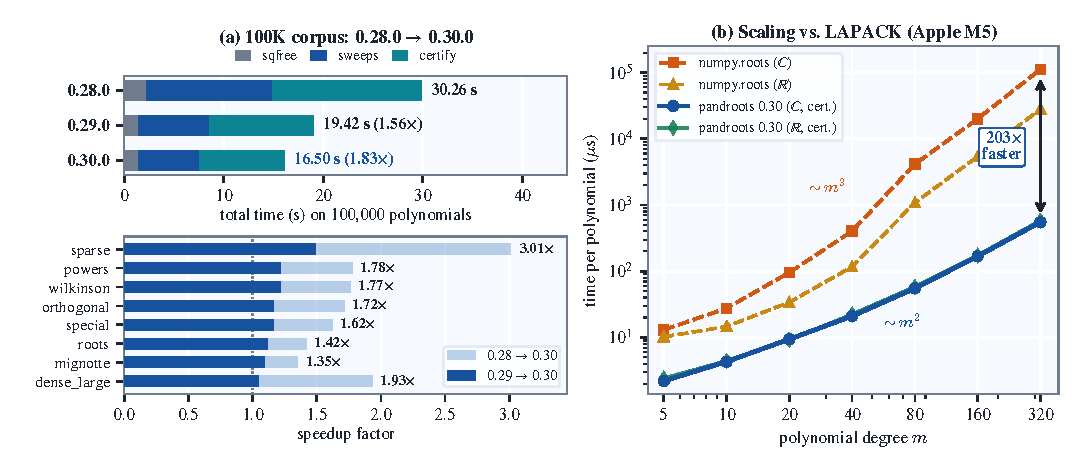
\includegraphics[width=\textwidth]{fig_bench.pdf}
\caption{Performance of \texttt{pandroots 0.30.0} on Apple~M5 (1 thread). (a)~Top: total runtime on the 100\,000-polynomial corpus across versions 0.28.0 (30.26\,s), 0.29.0 (19.42\,s), and 0.30.0 (16.50\,s, 1.83$\times$ faster overall), split into square-free decomposition, double-precision sweeps, and certification. Bottom: per-family speedups from 0.29.0$\to$0.30.0 (dark cobalt) and cumulative 0.28.0$\to$0.30.0 (light cobalt, reaching 3.01$\times$ on \texttt{sparse} and 1.93$\times$ on \texttt{dense\_large}). (b)~Log-log scaling from degree~5 to~320 against uncertified \texttt{numpy.roots}/LAPACK, exhibiting $O(m^2)$ vs.\ $O(m^3)$ growth and a 203$\times$ advantage at degree~320.}\label{fig:bench}
\end{figure}

% =========================================================================
\section{Clusters, zeros of $S'$, and local zoom}\label{sec:cluster}
Near a tight cluster of $K\ge2$ roots within $\rho$ of a centre $g$, simultaneous iterates at distance $d\gg\rho$ see one root of multiplicity $K$ and converge only linearly ($\frac14$ per sweep for a pair, $0.40$ for a triple, $\frac47$ for five roots). Three complementary mechanisms---all proposals judged afterwards by the same certificate of Section~\ref{sec:cert}---eliminate these stalls without altering Theorem~\ref{thm:g8}.

\subsection{The shifted-power cluster step (0.9.0, 0.10.0, 0.29.0)}
Seen from $d\gg\rho$, the cluster behaves like $(w-g)^K-a$, $|a|^{1/K}\approx\rho$: the $K$-th root model for which the rectangle with its exact support lands on all $K$ roots in one step~\cite{c5}.

\begin{proposition}\label{prop:cluster}
Let $f(w)=(w-g)^K-a$ with $K\ge2$, let $z$ be a point with $u=z-g\ne0$ and $f(z)\ne0$, and let $A=f'/f$, $B=(f'^2-ff'')/f^2$ at $z$. Then
\begin{equation}\label{eq:cluster}
 t=\frac{KB-A^2}{(K-1)A^2}=\frac{a}{u^K},\qquad \frac{K}{A\,(1-t)}=u,
\end{equation}
and the $K$ roots of $f$ are the points $g+u\,\omega$, $\omega^K=t$.
\end{proposition}
\begin{proof}
$f=u^K-a$, $f'=Ku^{K-1}$, $f''=K(K-1)u^{K-2}$, so $A=Ku^{K-1}/(u^K-a)$ and $B=Ku^{K-2}(u^K+(K-1)a)/(u^K-a)^2$. Then $KB-A^2=K^2(K-1)au^{K-2}/(u^K-a)^2$, giving $t=a/u^K$, $A(1-t)=K/u$, and $(u\omega)^K-a=0$.
\end{proof}

For a tight component $C$ of $K$ overlapping Smith discs (enclosing disc $\le\frac1{16}$ of its distance to outside discs), $S$ is deflated of the points \emph{outside} $C$ only, and when $|t|^{1/K}\le\frac14$ the $K$ points move to $z-u+u\,t^{1/K}\omega^j$. When $|t|<2^{-24}$, the cursor is read in multiprecision from $N,\beta$ with $K\log_2(d/r)+48$ bits of relative precision (0.10.0).

\textbf{Outermost-member fallback (0.29.0).}
If the first member of $C$ sits near the cluster centroid $g$, where $S'$ nearly vanishes or the model radius exceeds $\frac14|u|$, \texttt{cluster\_cursor} previously aborted. Since 0.29.0 it retries the remaining valid members of $C$ in decreasing order of Smith radius. On Mignotte triples $z^n-(a z-1)^3$ this single fallback drops multiprecision sweeps from 742 to 4 at $n=31$ and from 812 to 11 at $n=50$, both without zoom. When a whole factor remains in a single finite disc after refinement and zoom, version 0.28.0 retries once from \texttt{Start::Circle} and keeps the retry only if every root is isolated.

\subsection{Zeros of $S'$ (0.25.0) and local variable zoom beyond $2^{-500}$ (0.26.0)}
\textbf{Quadratic step at $S'=0$ (0.25.0).}
When two roots closer than $2^{-26}$ have a dyadic midpoint---such as $(z-1)(2^{40}z-2^{40}-1)$---double precision leaves both iterates at the zero of $S'$ between them, where $N=S/S'$ does not exist. In \texttt{refine\_for}, a point with $S'/S=0$ and $S\ne0$ now takes the quadratic step $h^2=-2S/S''$ away from its nearest neighbour, isolating $(z-1)(2^{40}z-2^{40}-1)$ in 3 sweeps at 128 bits instead of stalling to 4096 bits.

\textbf{Local zoom (0.26.0, module \texttt{zoom}).}
In \texttt{refine\_for}, ratios and distances are kept in double precision, so $S''/S$ overflows once two roots are closer than $\sim 2^{-500}$ of their modulus. Whenever a disc $D(z_0,R)$ still holds $K\ge2$ roots that should be separated, \texttt{zoom} introduces the local variable $u=2^m z - C$ with $2\le R\,2^m < 4$ and $C$ the nearest Gaussian integer to $2^m z_0$. The $K+1$ lowest-degree exact integer coefficients of $Q(u)=2^{mn}f((C+u)/2^m)$ form a degree-$K$ polynomial whose roots sit at distance $O(1)$ in $u$. Solving $Q$ (recursively if needed, up to depth 16) proposes $K$ points back in the variable of $f$, where they are certified globally by Theorem~\ref{thm:fp} using mantissa-exponent arithmetic and exact weight-ratio transfers $\prod_{i\in C}(z_l-z_i)/(z_l-z_i')$ for points outside $D(z_0,R)$ (\texttt{Zoom.lean}). Pairs $2^{-600}$ and $2^{-4000}$ apart are isolated into disjoint certified discs in 0.48--0.49\,ms (Table~\ref{tab:hp}, Figure~\ref{fig:zoom}); pairs $2^{-8000}$ apart are isolated in 30--80\,ms.

\begin{figure}[!htbp]\centering
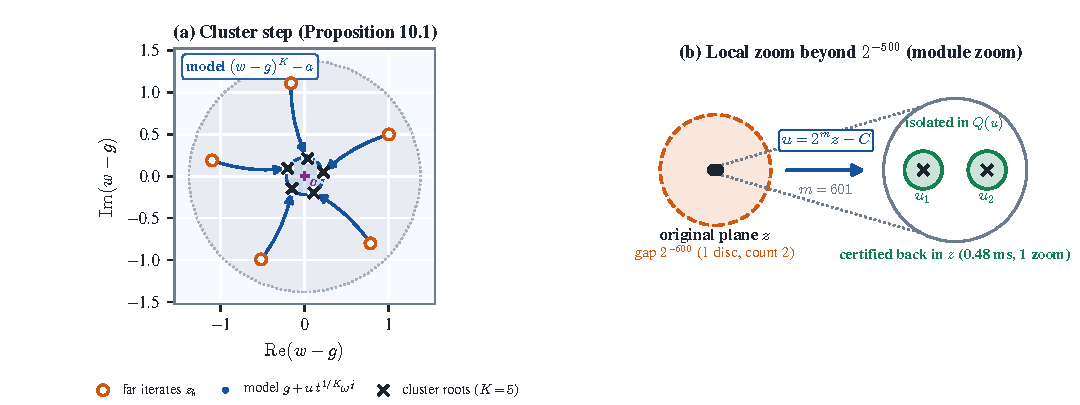
\includegraphics[width=\textwidth]{fig_zoom.pdf}
\caption{Cluster resolution at arbitrary scales. (a)~The shifted-power step (Proposition~\ref{prop:cluster}) maps five distant iterates straight onto the $K$-th root circle $g+u\,t^{1/K}\omega^j$ of the model $(w-g)^K-a$ in a single evaluation. (b)~Local variable zoom (module \texttt{zoom}, crate 0.26.0--0.30.0) rescales an unresolved cluster disc $D(z_0,R)$ via $u=2^m z-C$, isolates the roots at scale $O(1)$ in $Q(u)$, and certifies them back in the original variable $z$ (0.48\,ms for a $2^{-600}$ pair).}\label{fig:zoom}
\end{figure}

% =========================================================================
\section{Evidence and limits}\label{sec:evidence}

\textbf{Formalised in Lean~4} (Mathlib, toolchain v4.35.0; \textbf{10 modules, 84 theorems}, no \texttt{sorry}, standard axioms \texttt{propext}, \texttt{Classical.choice}, \texttt{Quot.sound} only; all files and SHA-256 build logs shipped in the \texttt{verification/lean} folder of the crate):
\begin{itemize}
\item \emph{Core G8 modules} (\texttt{SimultaneousRectangle}, \texttt{SmithDiscs}, \texttt{FixedPointCertificate}; 38 theorems): Proposition~\ref{prop:step}, Theorem~\ref{thm:order} cancellation identities and exact line~$AD$ bound (Remark~\ref{rem:ad}), $q_M(1)=1$, $q_M'(1)=\frac12$ and $q_2$; first half of Theorem~\ref{thm:smith}; Theorem~\ref{thm:fp} via Mathlib's contraction theorem; Corollary~\ref{cor:fp} down to the exact computed inequalities (\texttt{all\_roots\_of\_computed}); Proposition~\ref{prop:real} (\texttt{real\_disc\_of\_computed}); Proposition~\ref{prop:trap}.
\item \emph{Crate 0.6.0--0.10.0 modules} (31 theorems): \texttt{ZeroDeflation} (7 theorems), \texttt{FixedWidth} (4 lemmas), \texttt{ScaledVariable} (9 theorems), \texttt{ClusterStep} (6 theorems, Proposition~\ref{prop:cluster}), \texttt{ClusterCursor} (5 lemmas).
\item \emph{Multi-pass exact sweeps} (\texttt{SecondPass.lean}, 0.24.0; 5 theorems): with the other points on the other roots, the deflated sums leave only the target root's term, the cursor is $1$, $q_M(1)=1$ for every $p>1$, and every pass fixes the roots regardless of where $S$ was evaluated.
\item \emph{Local variable zoom} (\texttt{Zoom.lean}, 0.26.0; 10 theorems): change of variable $Q(u)=\kappa f((c+u)/d)$ preserves roots, multiplicities and single-root discs; exact Weierstrass weight-ratio update for unmoved points outside the cluster; disjoint single-root discs inside a $K$-root disc account for all $K$ roots.
\item \emph{Dyadic integer verifier} (\texttt{verification/dyadic}, 0.19.0--0.21.0): Aeneas-extracted Lean proofs of the separation scan, 128-bit dyadic rounding, and per-disc Rouch\'e acceptance in \texttt{src/disc\_check.rs}.
\end{itemize}

\emph{Not formalised:} the floating-point rounding bounds (Horner + underflow term, distance-product and sum margins), the fixed-point ball evaluation, the second half of Theorem~\ref{thm:smith} (Gershgorin's second theorem is not in Mathlib; used only as the fallback count on unresolved clusters), the quadratic step at $S'=0$, the C5 slit-plane branch arithmetic in floating point, the $O(m)$ V31 pre-polish, the fixed-width limb kernels (tested against \texttt{BigInt}), Yun's modular GCD (verified by exact division at runtime), and the Rust solver code itself.

\textbf{Written proofs and numerical validation.}
Written proofs cover Propositions~\ref{prop:step}, \ref{prop:real}, \ref{prop:trap}, \ref{prop:cluster}, Theorems~\ref{thm:order}, \ref{thm:smith}, \ref{thm:fp}, \ref{thm:g8}, Corollary~\ref{cor:fp}, and identity~\eqref{eq:precise}. In \texttt{pandroots 0.30.0}, all \textbf{80 tests} (29 unit tests, 46 integration tests across \texttt{basic}, \texttt{close\_roots}, \texttt{dyadic\_discs}, and 5 doctests) pass in release mode under both default features and \texttt{--features riemann-iterations}; on the 100\,000-polynomial corpus, all 36\,000 prescribed-root polynomials pass exact rational oracle verification with zero failures.

\textbf{Not new.}
Ehrlich--Aberth~\cite{ehrlich,aberth}; simultaneous Laguerre-type and Hansen--Patrick iterations of orders 4--6 with Newton/Halley neighbour corrections~\cite{hp,hpr,nourein,ppz,prp}; Smith's discs~\cite{smith}; Lagrange-form inclusion discs~\cite{bs,bh}; Newton-polygon starts~\cite{bini}; adaptive multiprecision and cluster restarts as in MPSolve~\cite{mpsolve}. Specific to this work: deriving the simultaneous sweep from the Pandrosion rectangle (Proposition~\ref{prop:step}), using the C5 slit-plane three-mean support $q_M(t)$ throughout (including $O(m)$ disjoint-disc pre-polish), the cancellation expansion of Theorem~\ref{thm:order}, the centroid-and-angle Newton-polygon start, the single-path exact-value / multi-pass / zoom escalation, the Lean~4 formalisation of the certificate and zoom chain, and the 100\,000-polynomial benchmark.

\textbf{Limits.}
\begin{itemize}
\item \emph{No theorem of global convergence:} as for Ehrlich--Aberth, convergence from the start is observed, not proved. Theorem~\ref{thm:g8} guarantees soundness of every output disc, not sharpness.
\item \emph{Order 9 does not transfer:} Remark~\ref{rem:nine} explains why the local order is 6 rather than 9. In compiled \texttt{pandroots 0.30.0}, the three-mean rectangle now beats Ehrlich--Aberth in wall-clock time at large degree (1.34$\times$ at degree~320), ties around degree~80, and trails slightly at degree~20 (Table~\ref{tab:sup_rust}).
\item \emph{Start and symmetric trap:} the binomial start loses to a single circle when all roots are grouped away from the origin (Table~\ref{tab:start}); the symmetric trap of Section~\ref{sec:trap} is escaped by rounding only.
\item \emph{Extreme clusters:} local zoom isolates dyadic and non-dyadic pairs down to $\sim 2^{-8000}$ apart, while non-dyadic clusters around $2^{-16000}$ (beyond 16 nested variable changes or $2^{26}$-bit local coefficients) remain grouped in one sound multi-root disc. On 5-root clusters, MPSolve remains ahead because evaluating $S$ near a 5-fold cluster requires five times the separation bits.
\item \emph{Single-threaded, safe Rust:} nothing runs in parallel and no \texttt{unsafe} SIMD intrinsics are used; timings come from one Apple~M5 machine and vary by 10--20\,\% across runs.
\end{itemize}

\begin{thebibliography}{99}\small
\bibitem{aberth} O.~Aberth. Iteration methods for finding all zeros of a polynomial simultaneously. \emph{Math. Comp.} 27 (1973), 339--344.
\bibitem{bs} W.~B\"orsch-Supan. Residuenabsch\"atzung f\"ur Polynom-Nullstellen mittels Lagrange-Interpolation. \emph{Numer. Math.} 14 (1970), 287--296.
\bibitem{bh} D.~Braess, K.~P.~Hadeler. Simultaneous inclusion of the zeros of a polynomial. \emph{Numer. Math.} 21 (1973), 161--165.
\bibitem{bini} D.~A.~Bini. Numerical computation of polynomial zeros by means of Aberth's method. \emph{Numer. Algorithms} 13 (1996), 179--200.
\bibitem{mpsolve} D.~A.~Bini, L.~Robol. Solving secular and polynomial equations: a multiprecision algorithm. \emph{J. Comput. Appl. Math.} 272 (2014), 276--292.
\bibitem{v31} I.~Besevic. \emph{Geometric Root Calculators}, version V31, 2026.
\bibitem{c5} I.~Besevic. \emph{Complex Geometric Root Calculators}, version C5, 2026.
\bibitem{g2} I.~Besevic. \emph{Geometric Root Calculators for arbitrary polynomials: the anchored rectangle}, version G2, 2026.
\bibitem{g3} I.~Besevic. \emph{A globally convergent geometric calculator for every complex polynomial}, version G3, 2026.
\bibitem{g5} I.~Besevic. \emph{All real roots, with their multiplicities}, version G5, 2026.
\bibitem{g6} I.~Besevic. \emph{All the roots of a polynomial, with their multiplicities}, version G6, 2026.
\bibitem{g7} I.~Besevic. \emph{Find, certify, count}, version G7, 2026.
\bibitem{ehrlich} L.~W.~Ehrlich. A modified Newton method for polynomials. \emph{Comm. ACM} 10 (1967), 107--108.
\bibitem{gersh} S.~Gerschgorin. \"Uber die Abgrenzung der Eigenwerte einer Matrix. \emph{Izv. Akad. Nauk SSSR} 7 (1931), 749--754.
\bibitem{hp} E.~Hansen, M.~Patrick. A family of root finding methods. \emph{Numer. Math.} 27 (1977), 257--269.
\bibitem{hpr} E.~Hansen, M.~Patrick, J.~Rusnak. Some modifications of Laguerre's method. \emph{BIT} 17 (1977), 409--417.
\bibitem{higham} N.~J.~Higham. \emph{Accuracy and Stability of Numerical Algorithms}, 2nd ed. SIAM, 2002.
\bibitem{nourein} A.-W.~M.~Nourein. An improvement on two iteration methods for simultaneous determination of the zeros of a polynomial. \emph{Int. J. Comput. Math.} 6 (1977), no.~3.
\bibitem{ppz} M.~S.~Petkovi\'c, L.~D.~Petkovi\'c, D.~\v{Z}ivkovi\'c. Laguerre-like methods for the simultaneous approximation of polynomial zeros. In \emph{Topics in Numerical Analysis}, Computing Supplementum 15, Springer, 2001.
\bibitem{prp} L.~D.~Petkovi\'c, L.~Ran\v{c}i\'c, M.~S.~Petkovi\'c. An efficient higher order family of root finders. \emph{J. Comput. Appl. Math.} (2008), 56--72.
\bibitem{smith} B.~T.~Smith. Error bounds for zeros of a polynomial based upon Gerschgorin's theorems. \emph{J. ACM} 17 (1970), 661--674.
\bibitem{traub} J.~F.~Traub. \emph{Iterative Methods for the Solution of Equations}. Prentice-Hall, 1964.
\end{thebibliography}
\end{document}
